% !TeX root = ../libro.tex
% !TeX encoding = utf8


\chapter{Resultados de frenado magnético de intensidad fija}\label{ch:quinto-capitulo}
\section{Configuración de los modelos} \label{marco_teorico}
A COMENTAR
Parametrización de los modelos
Rango de valores a asignar a los parámetros libres
Ciclo de control
Para cada paso de simulación
- Obtenemos o calculamos la intensidad del campo magnético
- Calculamos la pérdida de momento angular inducida por el campo magnético
- Distribuimos la pérdida de momento angular entre las capas de la estrella
- Obtenemos o calculamos el valor de $\amlt$


\section{Modelos de evolución estelar}
De acuerdo con la formulación de las secciones anteriores, los dos únicos parámetros libres de nuestra implementación son $B$ y $\Omega$. Las simulaciones numéricas trazaron la historia rotacional y $A(\isotope[7]{Li})$ de una estrella 1 $\msun$ para una variedad de valores iniciales para $B$ y $\Omega$ (ver también Tabla \ref{tab:phy_mesa}). MESA utiliza el enfoque en capas (shellular) \cite{Meynet1997} para dar cuenta de los efectos hidrostáticos de la rotación en modelos estelares 1D.\par


\begin{table}
	\centering
	\caption{Summary of adopted physics in MESA \cite[based on][]{Choi2016}.}
	\label{tab:phy_mesa}
	\begin{tabular}{ll} 
		\hline
		Parameter & Adopted prescriptions and values\\
		\hline
		Solar Abundance & $X_{\odot}=0.7154, Y_{\odot}=0.2703, Z_{\odot}=0.0142$\\
		Equation of State & OPAL+SCVH+MacDonald+HELM+PC\\
		Opacity & OPAL Type I for log T $\geq$ 4 \\ & Ferguson for logT $\leq$ 4\\
		Reaction Rates & JINA REACLIB\\
		Boundary Conditions & ATLAS12; $\tau$=100 tables + photosphere\\
		Difussion & Track \isotope[1]{H}, \isotope[2]{He}, \isotope[7]{Li}, \isotope[7]{Be}\\
		Rotation & Differential rotation at PMS \& MS\\
		Convection & MLT + Ledoux, $\alpha_{MLT}$ = 1.82\\
		Overshoot & time-dependent, diffusive, \\ & $f_{ov,core}=0.0160$,\\ 
		& $f_{ov,sh}=0.0174$\\
		Semiconvection & $\alpha_{sc}=0.1$\\
		Thermohaline & $\alpha_{th}=666$\\
		Rotational Mixing & Include SH, ES, GSF, SSI \& DSI\\
		Magnetic Effects & Magnetic braking based on idealized \\ & monopole field\\
		Magnetic Field & B(G) variable between [3.0 - 5.0]\\
		Mass Loss & activated, $\Dot{M}_{max} = 10^{-3} \: \msun \: yr^{-1}$\\
		Angular Moment Loss & activated, $\Dot{J} = \frac{2}{3} \Dot{M}\Omega R^{2}_{A}$\\
		\hline
	\end{tabular}
\end{table}

Adoptamos abundancias a escala solar y asumimos una abundancia inicial solar ($Z = Z_{\odot, \mathrm{pr} = 0,0142}$). También adoptamos los siguientes valores nominales para expresar las propiedades estelares en unidades SI, $\rsun = 6,957x10^{10}\, cm$ y $\msun = 1,988x10^{33}\, g$ que son coherentes con las resoluciones de la IAU \cite{Mamajek2015}. Para una descripción detallada de la física adoptada en este trabajo, remitimos al lector a \cite{Choi2016}. Ese trabajo se utilizó como punto de partida para el nuestro en lo que respecta a la parametrización del proyecto MESA, que se calibró para reproducir las abundancias de elementos medidas en la superficie solar.\par

Los modelos incluyeron la rotación durante la PMS ya que existen evidencias que abogan por una fuerte relación establecida entre la destrucción de Li y la rotación en esa fase (\cite{Bouvier2016,Bouvier2018}). Modelamos la rotación como AML se calcula como resultado del par aplicado a la zona de convección por un viento acoplado magnéticamente. Además, no tuvimos en cuenta ni la influencia de los campos magnéticos internos ni su existencia durante la fase T-Tauri.\par 
---CORREGIR ESTO SEGUN EL NUEVO PAPERAdoptamos un enfoque teórico sencillo y pragmático para establecer cuándo la estrella está alcanzando la fase ZAMS. El criterio elegido se basó en la existencia simultánea de una extensa capa convectiva y un núcleo radiativo. A partir de este momento, se activó la rutina MB, actuando como un mecanismo adicional a los existentes en el código evolutivo MESA que participó en el AML de la estrella. ---HASTA AQUÍ---\par

Supusimos que el campo magnético no variaba su intensidad a lo largo de la evolución de la estrella hasta alcanzar el TAMS. Además, también se consideraron otros efectos de rotación durante la evolución de los modelos: el transporte de AM desde el interior radiativo hasta la envoltura convectiva y la redistribución de AM asociada a cambios en la estructura interna durante el proceso de contracción hacia la EM.\par

Nos centramos en el papel indirecto que desempeña el MB en la destrucción del Li. Esto es consecuencia de su influencia en la historia rotacional de las estrellas de tipo solar. Nuestro principal objetivo era comprobar cómo el MB podría contribuir a explicar la evolución del Li en el Sol y en otras estrellas de tipo solar. Se ejercitaron un conjunto de escenarios diferentes con intensidades de campo magnético que oscilaban entre 3,0 y 5,0 G. Calculamos la evolución de modelos estelares 1 $\msun$ con metalicidad inicial solar y $\oomegac$ variable entre $0.0084$ y $0.0336$. Los modelos más avanzados para disposiciones más complejas del campo magnético, así como la evolución de su intensidad a lo largo de la vida de la estrella, se dejaron para trabajos posteriores.\par

Como expresa la Ec.~\ref{eq:j_dot_mesa}, la cantidad de AML depende de $R_A$ (o alternativamente de $\eta_*$), $\Omega$ y $\Dot{M}$. Para un valor grande de $\eta_*$, la estrella experimenta una desaceleración significativa. Controlamos el valor de $\eta_*$ en los modelos variando el campo magnético ($B$) y la velocidad de rotación estelar ($\Omega$). Con respecto a $\Dot{M}$ y como se indica en la tabla \ref{tab:phy_mesa}, para calcular la pérdida de masa se utilizó la fórmula empírica desarrollada por Reimers \cite{Reimers1975} para estrellas en la rama gigante asintótica (AGB). Para una estrella de tipo solar el $\Dot{M}$ durante la EM es relativamente pequeño, alrededor de $10^{-14}\msun \, yr^{-1}$ \cite{Noerdlinger2008}. \par

\subsection{Evolución de Li sin MB}

\begin{figure}
    \centering
	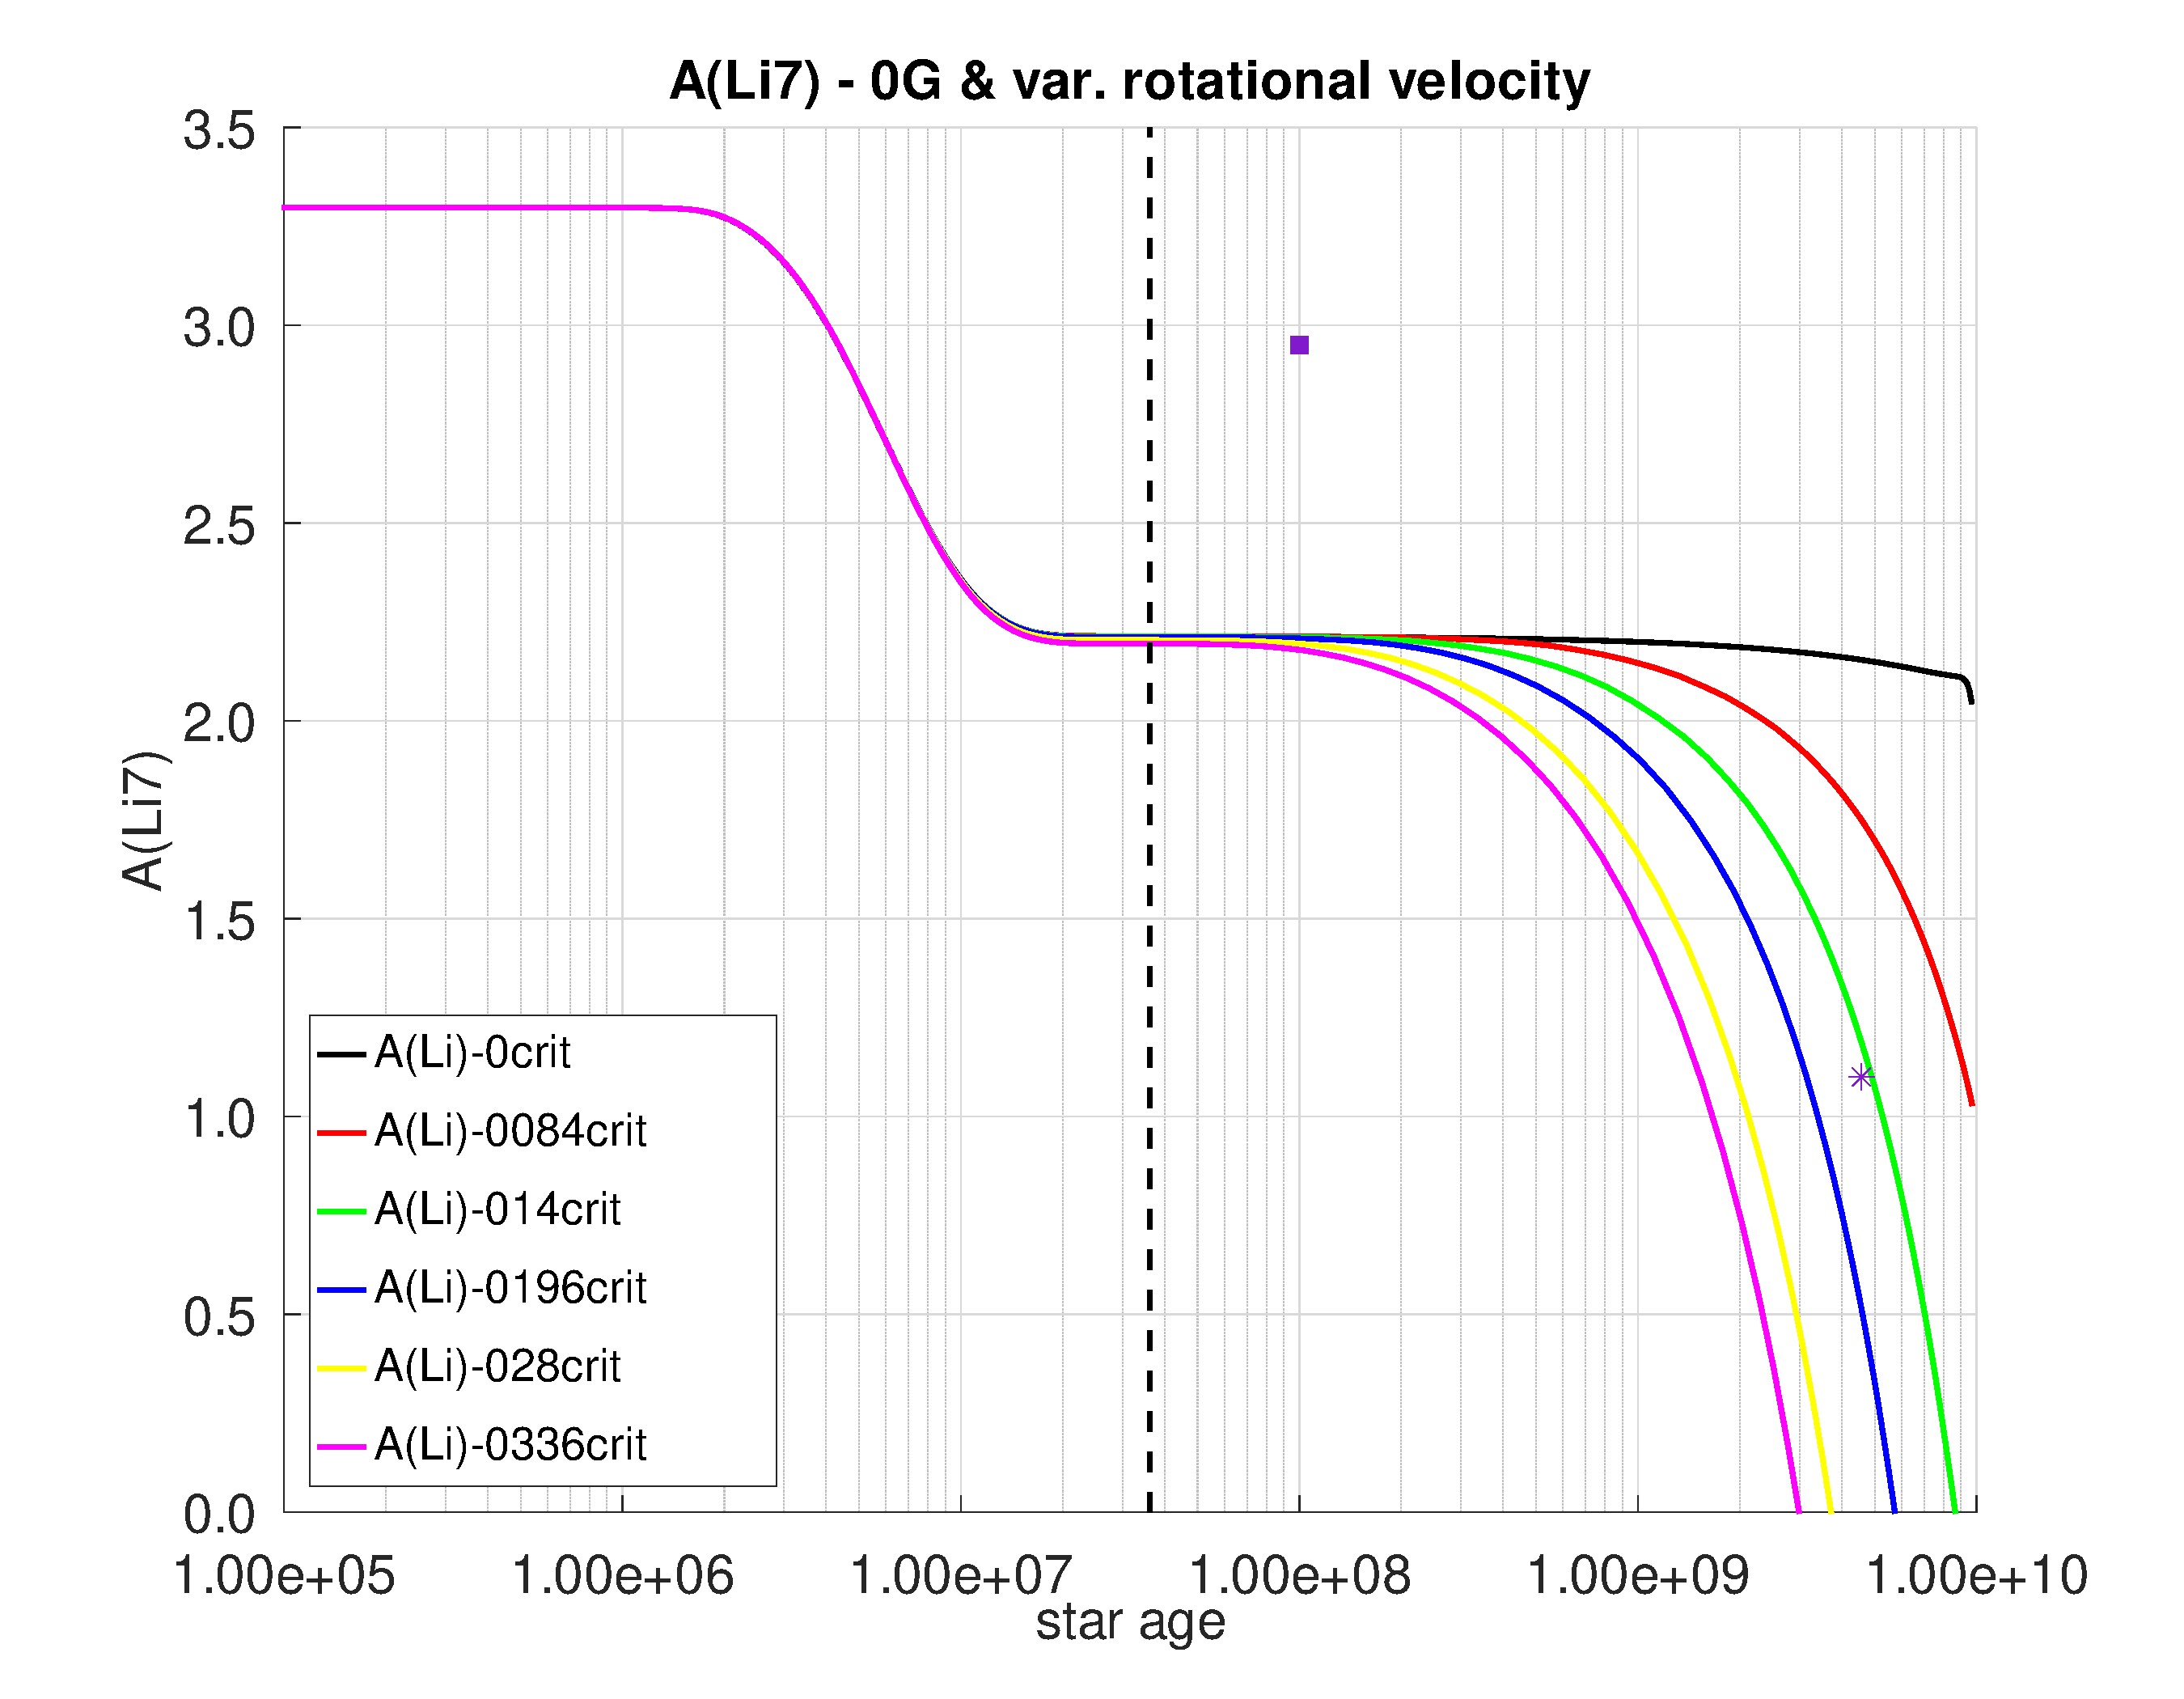
\includegraphics[width=0.7\textwidth]{img/paper1/li_var_vel_0_0g.pdf}
	\caption{La evolución de la abundancia superficial del \isotope[7]{Li} en relación con el \isotope[1]{H}, en función del tiempo para varios modelos de 1 $\msun$. La línea negra continua representa el modelo de referencia según \cite{Choi2016}. El resto de líneas son modelos que incluyen rotación PMS con $\oomegac$ entre 0.0084 y 0.0336, respectivamente. La estrella púrpura y el cuadrado son abundancias superficiales de Li para el Sol actual \cite{Asplund2009} y la media para el cúmulo de las Pléyades \cite{Sestito2005} respectivamente. La línea vertical discontinua hace referencia a la ZAMS.}
	\label{fig:li_var_vel_0g}
\end{figure}

La figura \ref{fig:li_var_vel_0g} muestra la evolución temporal de la abundancia superficial de Li para varios modelos $1\msun$ inicializados con diferentes velocidades de rotación. Las simulaciones tuvieron en cuenta los efectos de rotación y AML causados por los vientos estelares pero no los de MB. La estrella púrpura y el cuadrado son las abundancias superficiales de Li para el Sol actual \cite{Asplund2009} y para las Pléyades, respectivamente \cite{Sestito2005}.\par

Obsérvese cómo la abundancia de Li en la superficie estelar disminuyó con el tiempo para todos los modelos simulados. La línea negra continua representa el modelo de referencia que adopta los parámetros de superación de la envoltura calibrados para el Sol, como se documenta en \cite{Choi2016}. Todos los modelos quemaron demasiado Li antes de la ZAMS y, por tanto, no coincidieron con la abundancia media de Li en superficie de las Pléyades. También fue destacable el hecho de que apenas hubo diferencias entre los distintos modelos en cuanto a la abundancia de Li durante gran parte de la ZAMS. Sólo después de un millón de años se destruyó el Li en un grado acentuado, ya que antes no se alcanzó la temperatura necesaria en BCZ. Después, los diferentes modelos destruyeron el Li de forma muy similar debido a dos razones principales. Por un lado, las zonas convectivas que desarrollaron los modelos tenían tamaños muy similares, por lo que la temperatura en la BCZ era prácticamente la misma. Por otro lado, el diferencial de rotación entre el núcleo y la zona convectiva no comenzó a desarrollarse hasta que alcanzó los $ \approx 10^6$ años, alcanzando su máxima diferencia en la ZAMS alrededor de los $ \approx 10^7$ años. Fue en este momento cuando debieron aumentar los efectos combinados de la turbulencia y la diferencia rotacional, dando lugar a notables diferencias en la evolución de A(Li) (véase la figura \ref{fig:li_var_vel_0g_z1}). Posteriormente, el modelo de referencia (línea negra) no agotó eficientemente el Li en la EM y no consiguió (de nuevo) igualar la abundancia actual de Li en la superficie solar. Los otros modelos que incluían la rotación durante el PMS con valores de $\oomegac$ entre 0.0084 y 0.0336 fueron capaces de quemar Li de forma más realista. Entre ellos, sólo uno (línea verde) se aproximaba a la abundancia actual de Li del Sol, pero su velocidad de rotación era mucho mayor (véase la figura \ref{fig:rot_vel_0g}) que los $2\,\kms$ del Sol \cite{Gill2012}. \par

Durante gran parte del PMS la estrella giró como un cuerpo sólido (véase la Figura \ref{fig:rot_vel_0g}) y esto se debió a que la estrella tenía un interior totalmente convectivo. No fue hasta el final de la trayectoria de Hayashi cuando la estrella comenzó a desarrollar un núcleo radiativo. Fue en esta etapa cuando apareció una diferencia de velocidad angular entre los límites superior e inferior de las zonas radiativa y convectiva respectivamente. El grado de rotación diferencial estaba directamente influido por la $\Omega$ inicial. A medida que los modelos se inicializaban con una velocidad angular mayor, se acentuaba la diferencia de velocidad entre la BCZ y la superficie estelar; cuanto mayor era la velocidad inicial, mayor era el gradiente de velocidad entre los límites inferior y superior de la CZ. Como consecuencia, la fuerza de la turbulencia localizada en la BCZ aumentó, de modo que el Li pudo alcanzar regiones con temperaturas cercanas a $\tli$, donde finalmente se quemó y destruyó (véase la figura \ref{fig:li_var_vel_0g}). Otras investigaciones \cite{Bouvier2018, Baraffe2017} apuntan a una tendencia diametralmente opuesta a la aquí expuesta, es decir, a mayor velocidad de rotación, mayor abundancia de Li en la superficie de la estrella. \par

\begin{figure}
    \centering
    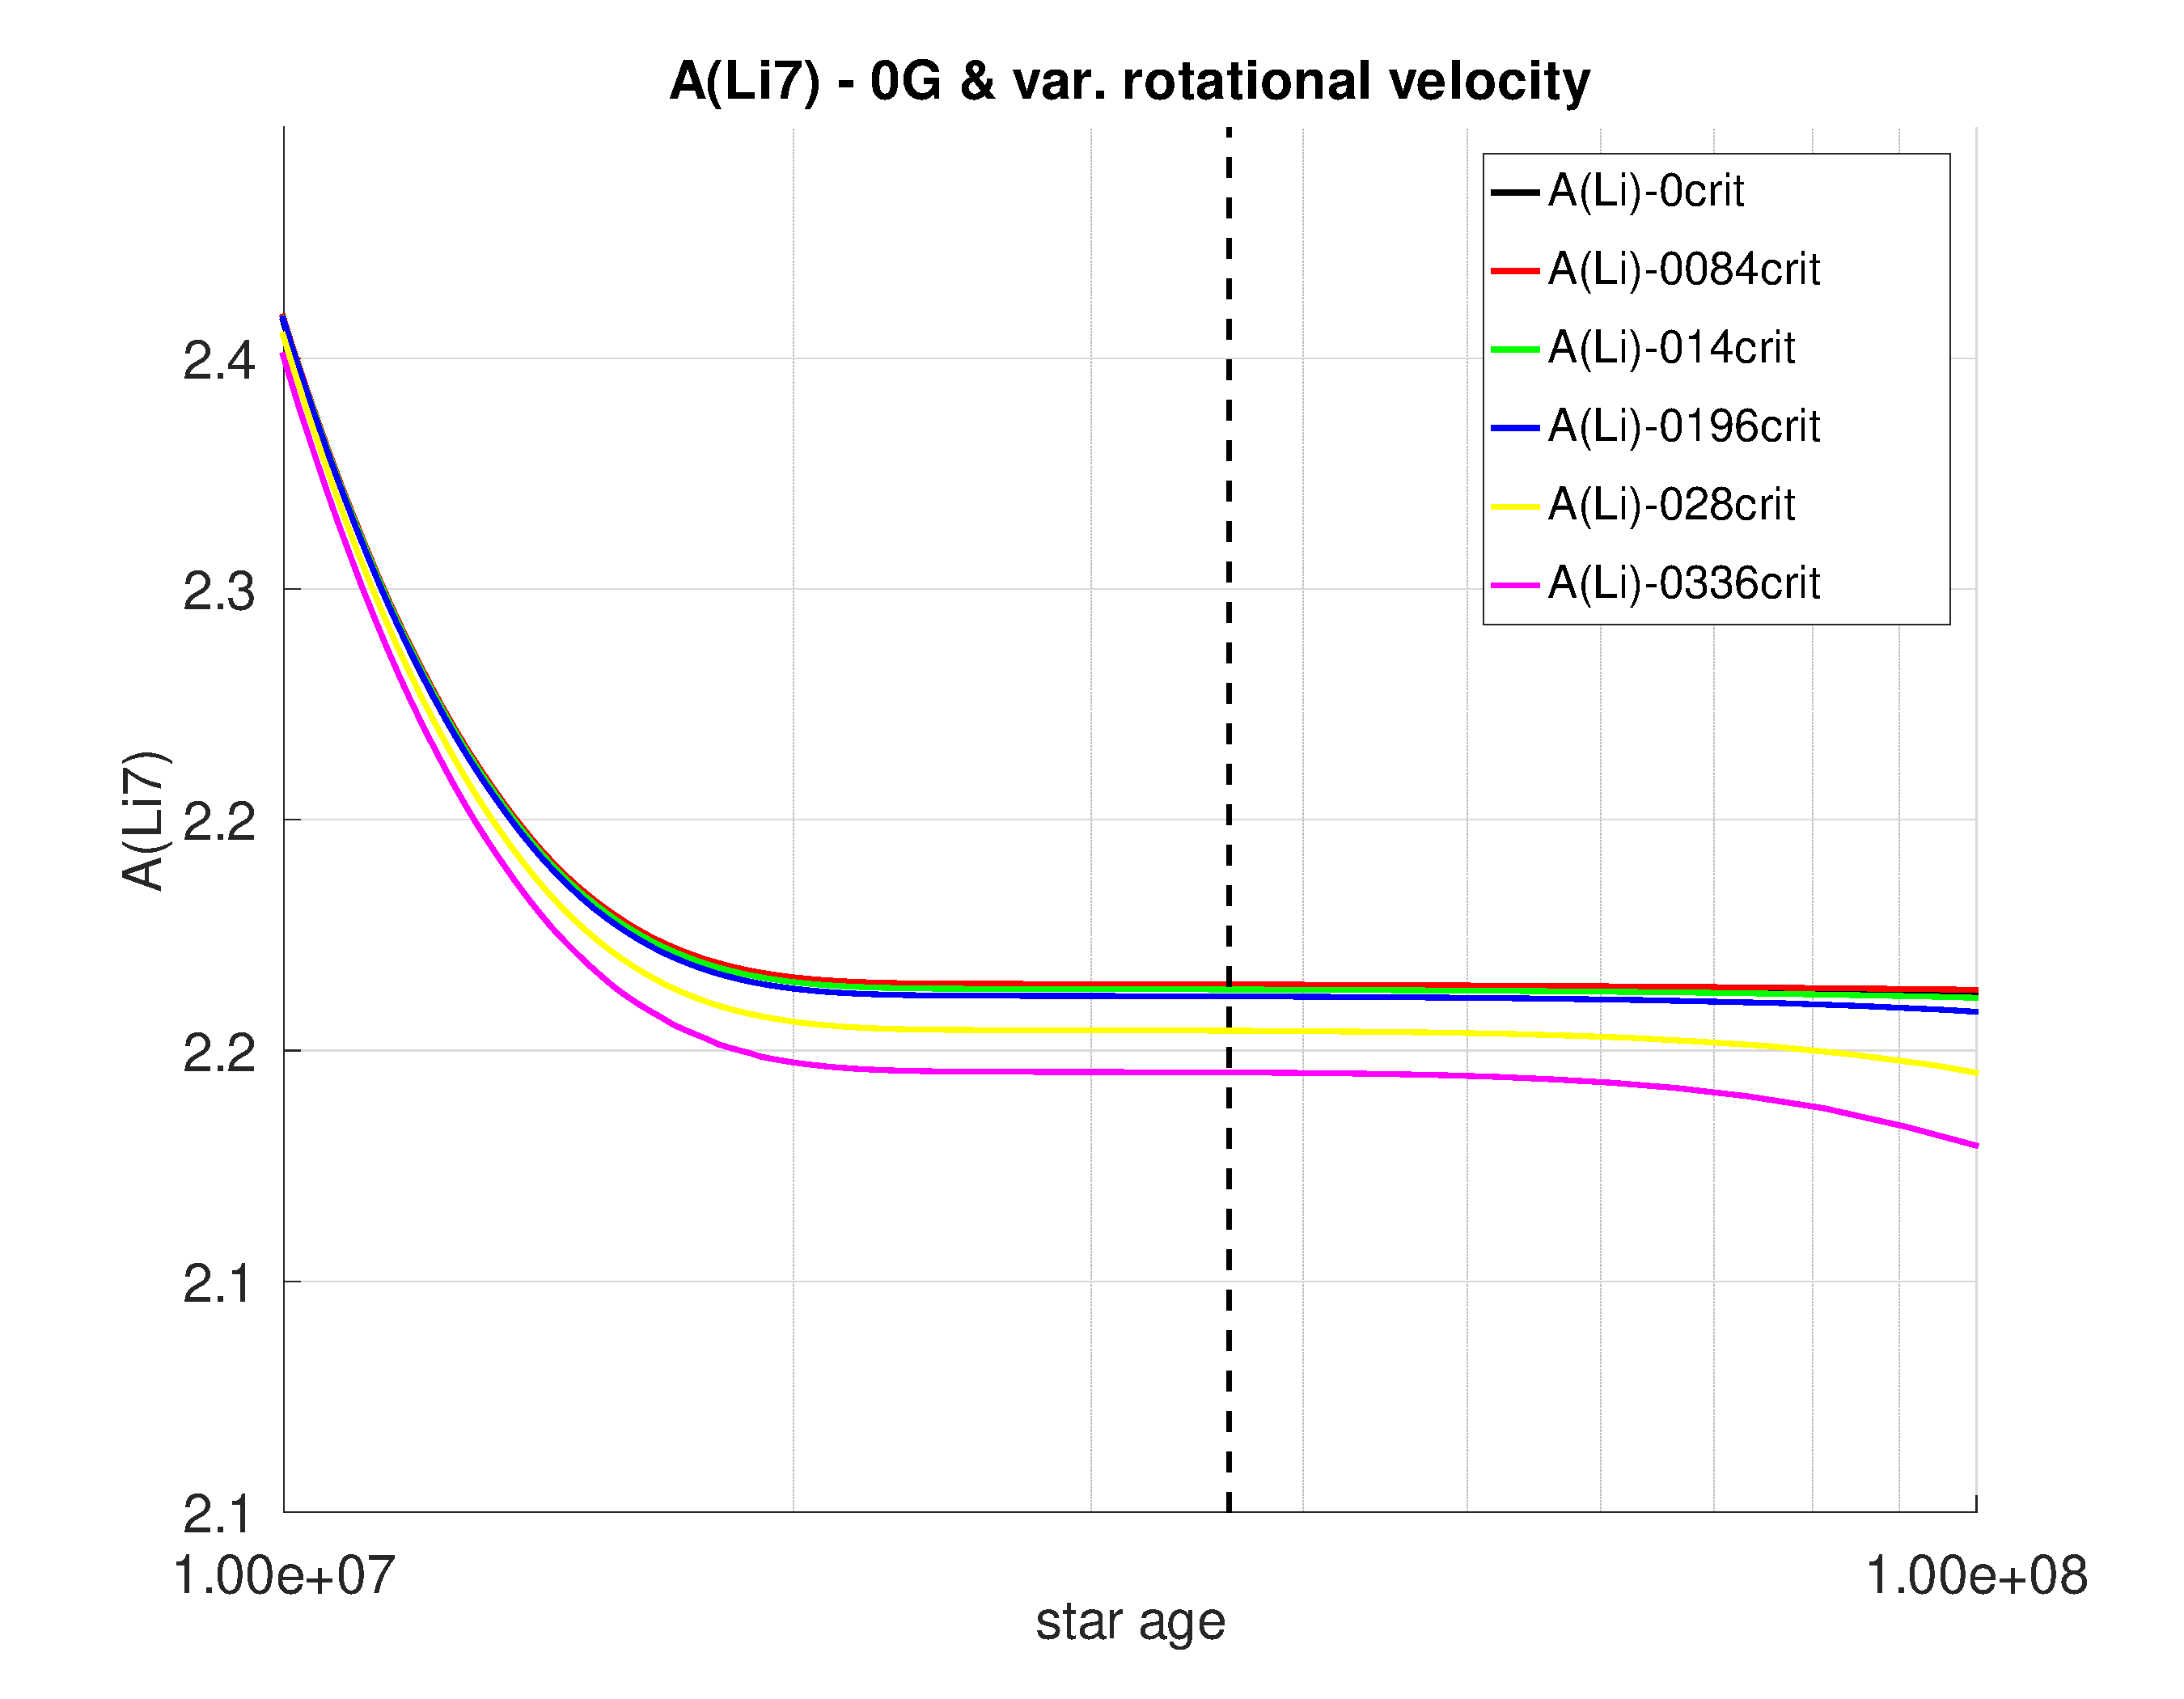
\includegraphics[width=0.7\textwidth]{img/paper1/li_var_vel_0_0g_z1.pdf}
	\caption {Similar a la Figura \ref{fig:li_var_vel_0g} pero ampliando la ZAMS. Los modelos con una mayor velocidad de rotación inicial alcanzan ya la ZAMS con una menor cantidad de medida de Li en la superficie estelar.}
	\label{fig:li_var_vel_0g_z1}
\end{figure}

\begin{figure}
	\centering
	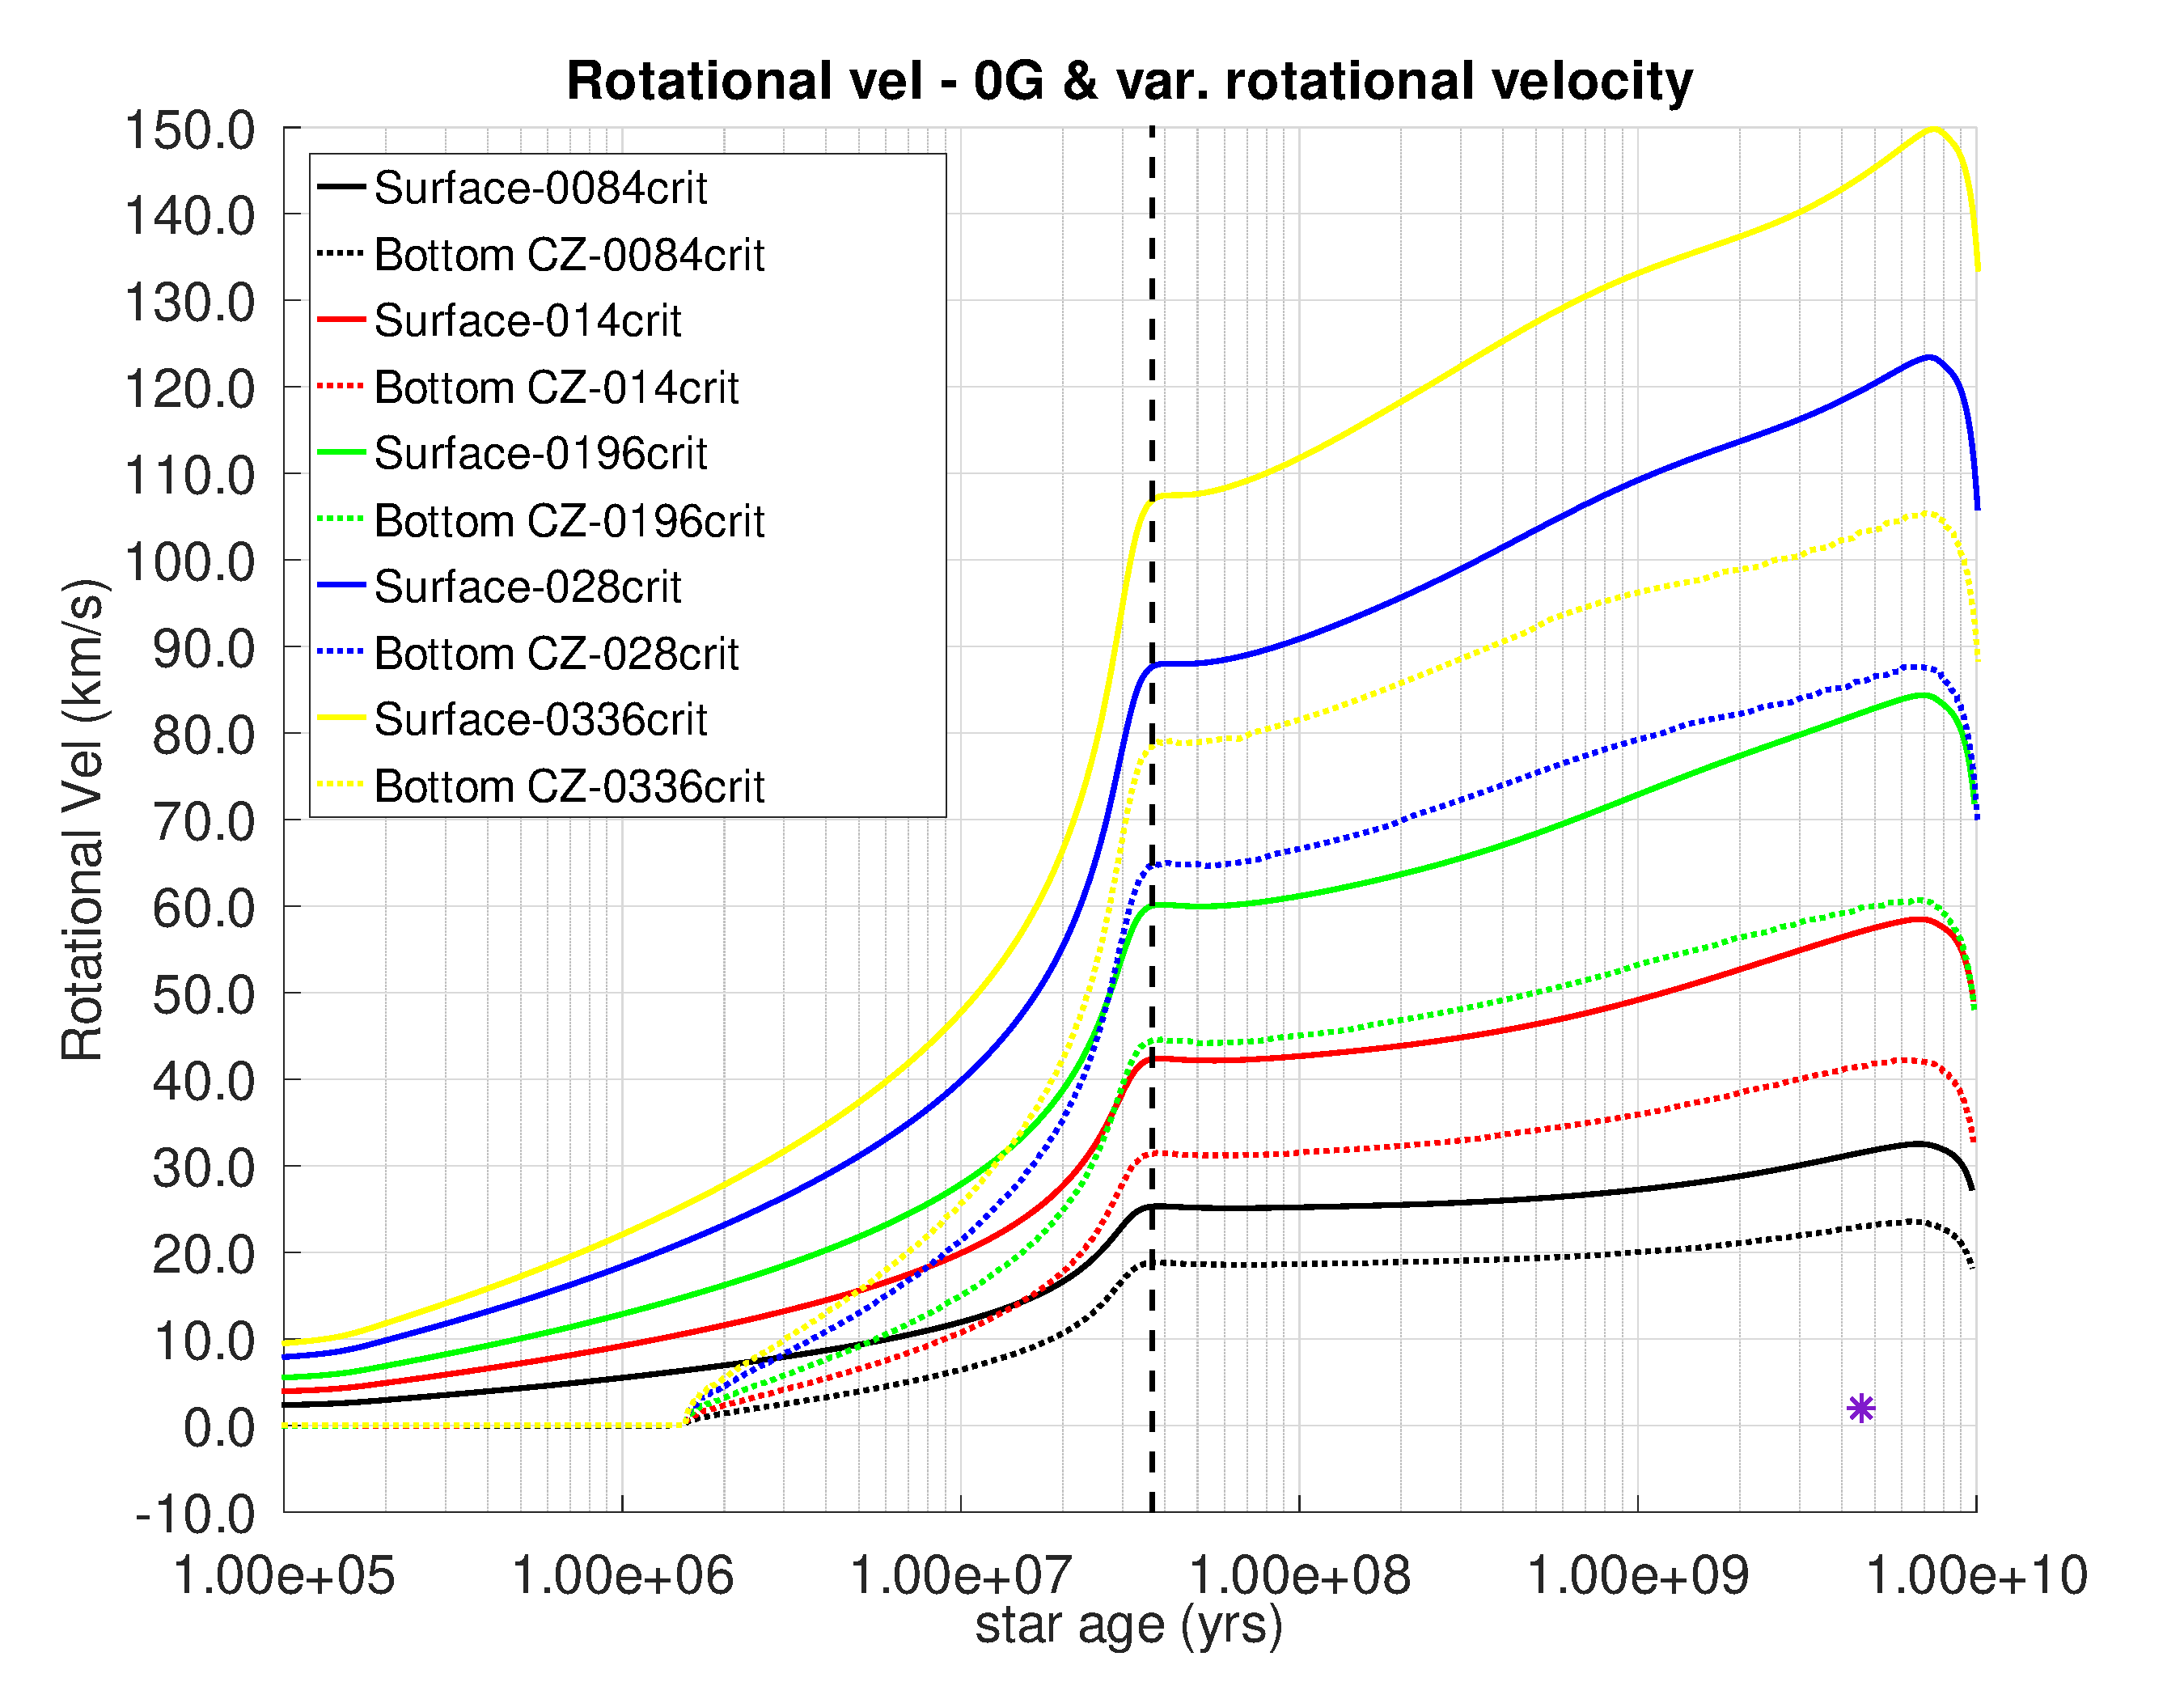
\includegraphics[width=0.7\textwidth]{img/paper1/rot_vel_var_vel_0_0g.pdf}
	\caption{Evolución de la velocidad angular en la superficie (línea continua) y en el límite inferior (línea discontinua) de la zona convectiva superior, en función del tiempo para varios modelos de 1 $\msun$. Los modelos incluyen rotación PMS con valores $\oomegac$ entre 0,0084 y 0,0336. La estrella púrpura es la velocidad angular superficial para el Sol actual \cite{Gill2012}. La línea vertical discontinua hace referencia a la ZAMS.}
	\label{fig:rot_vel_0g}
\end{figure}

Otros efectos estructurales bien conocidos de la rotación son la disminución de la temperatura efectiva ($\teff$) y, en menor medida, de la luminosidad estelar ($L$). Ambos efectos pueden observarse gráficamente en el diagrama HR de la figura \ref{fig:hr_var_vel_0g}, que muestra una vista ampliada de las trayectorias evolutivas desde la ZAMS hasta la TAMS para varios modelos $\msun$ inicializados con diferentes velocidades de rotación. Si comparamos el modelo no rotatorio (línea sólida negra) con los rotatorios podemos reconocer que al final del PMS, estos últimos alcanzan la ZAMS con un $\teff$ menor que los primeros. Estos resultados coinciden con los de estudios anteriores \cite[véase por ejemplo ][]{Eggenberger2012,Piau2001,Pinsonneault1989}.\par

\begin{figure}
    \centering
    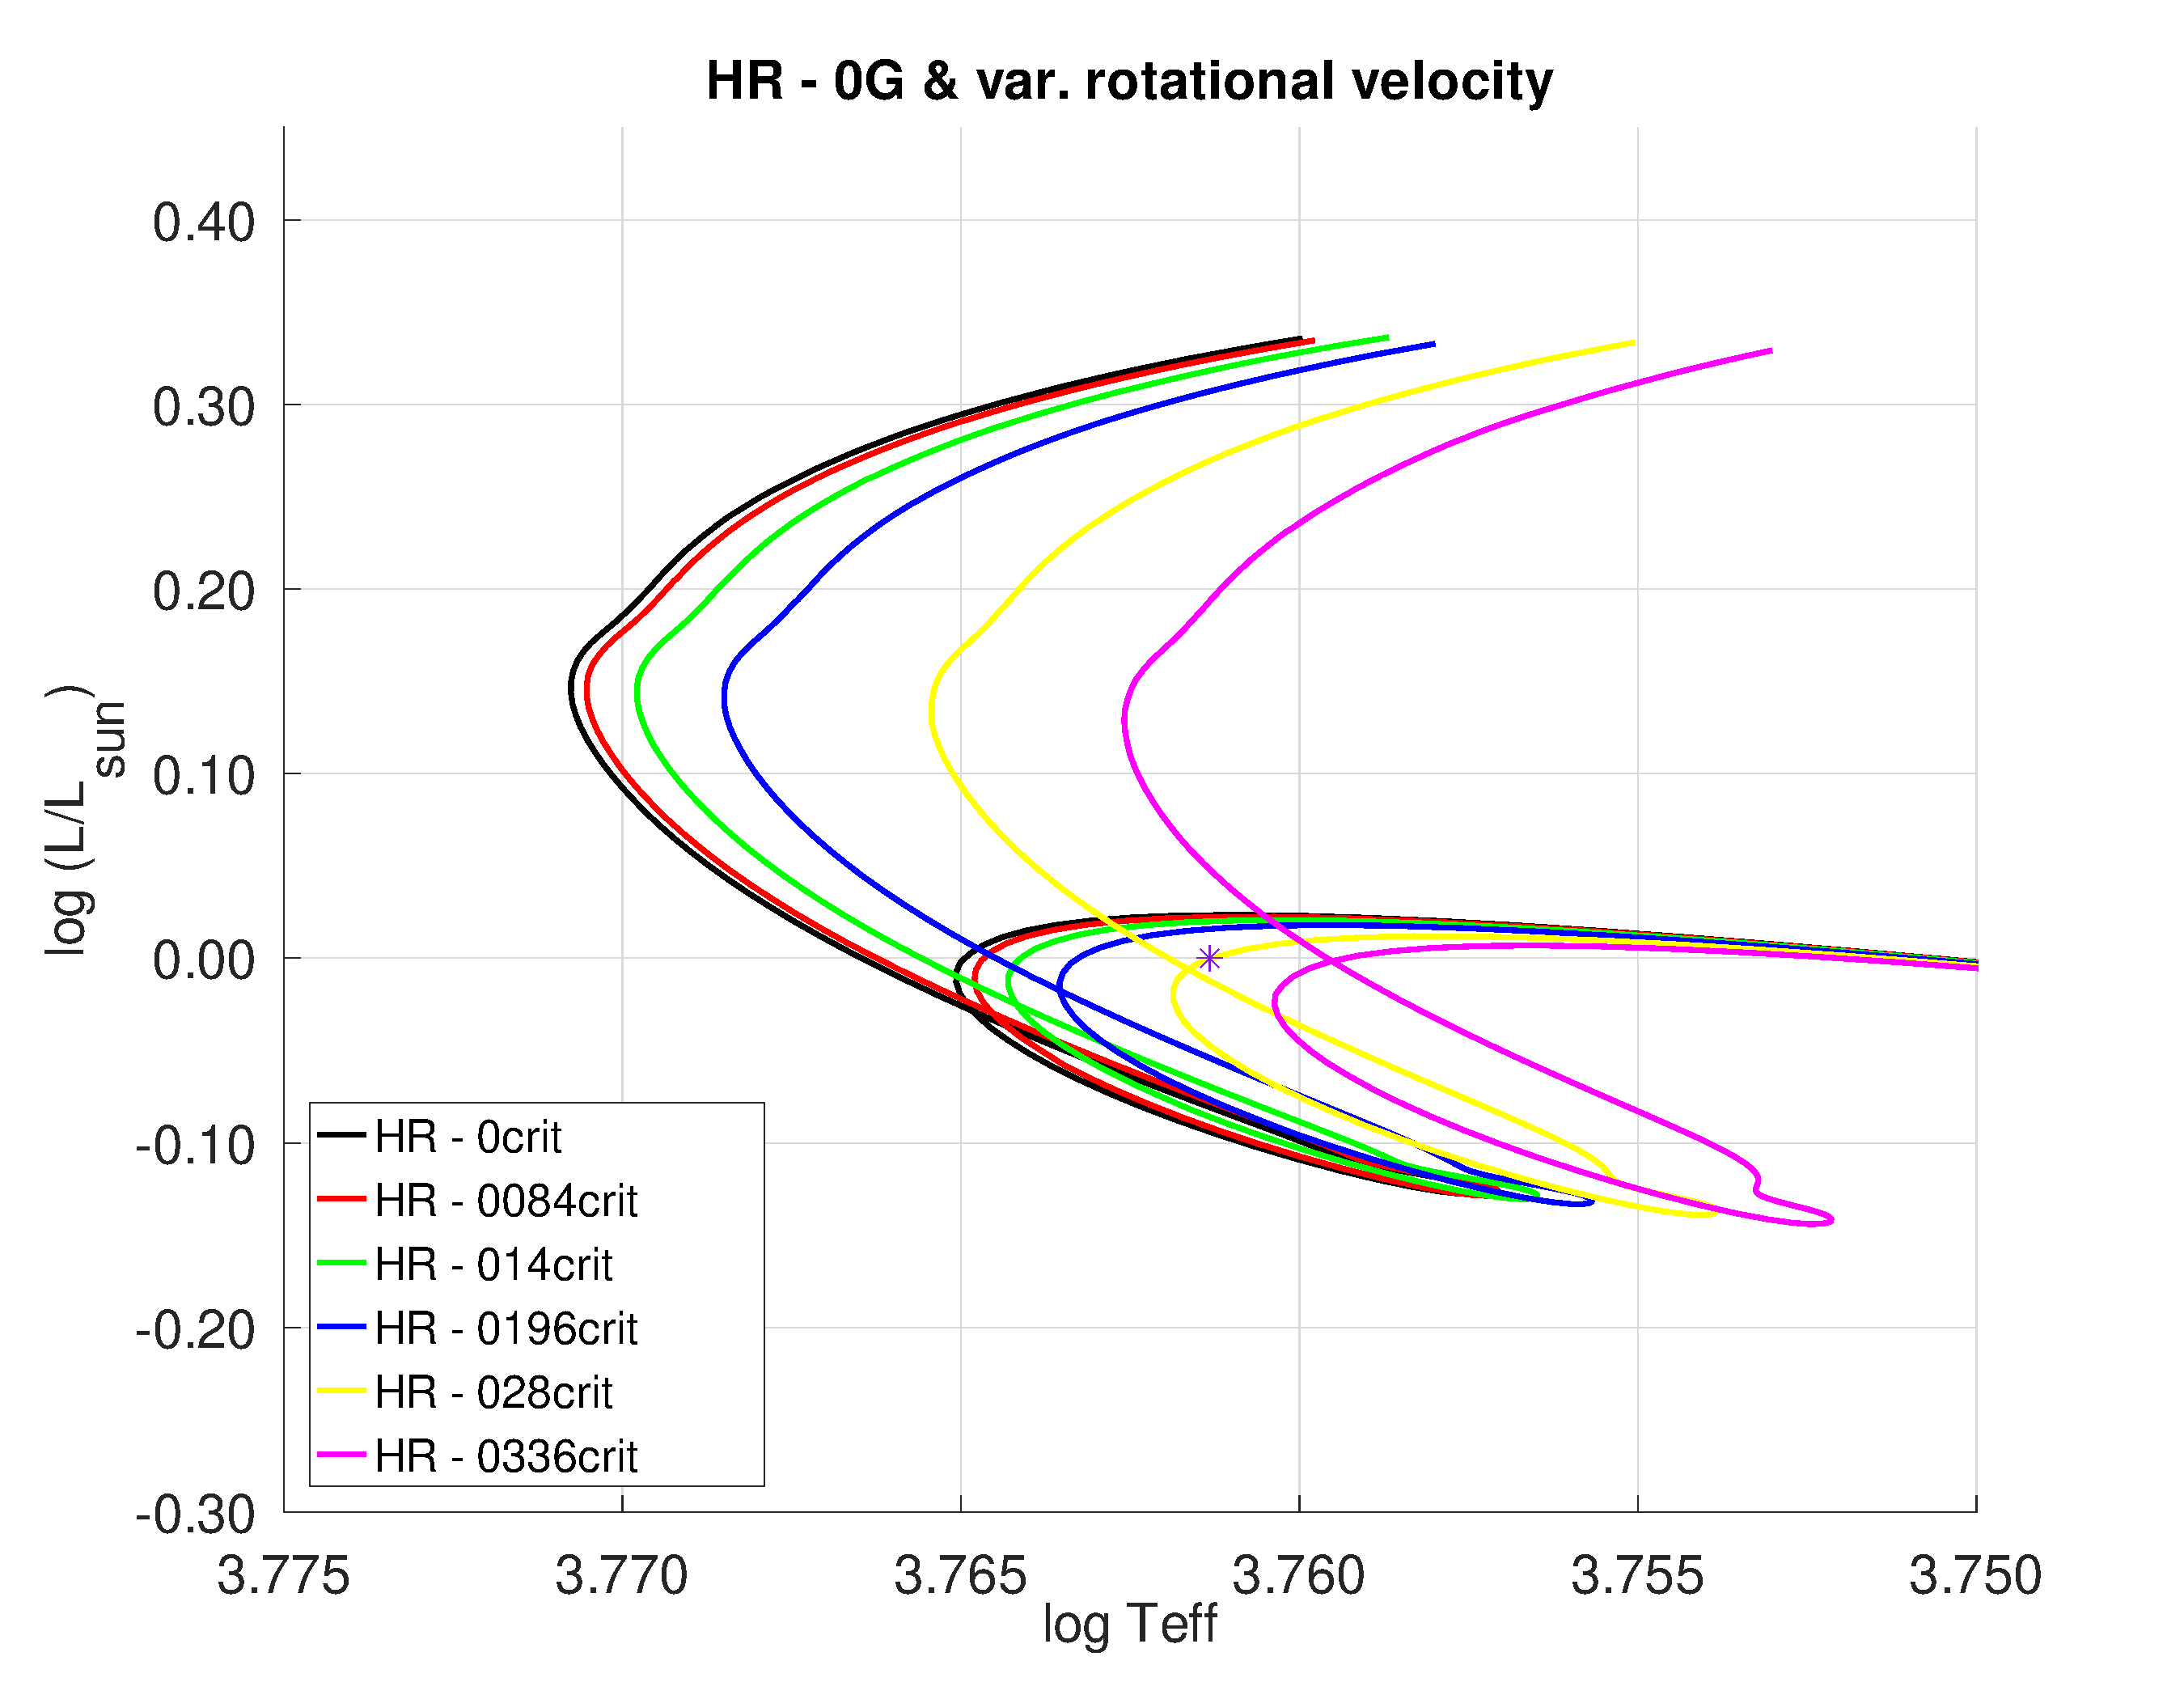
\includegraphics[width=0.7\textwidth]{img/paper1/hr_var_vel_0_0g_z1.pdf}
	\caption{Un ejemplo de cuadrícula solar de 1$\msun$ de trayectoria evolutiva estelar desde el PMS hasta el TAMS cubriendo un amplio rango de velocidades angulares. La rotación se activa en los modelos en el PMS y esos modelos llegan antes a la ZAMS y a un $\teff$ menor que el de no rotación (línea negra continua). La luminosidad se expresa en términos de $\lsun$.}
	\label{fig:hr_var_vel_0g}
\end{figure}

\subsection{Evolución del Li con MB de intensidad fija}
La figura \ref{fig:li_var_vel_4_0g} muestra la evolución temporal de la abundancia superficial de Li para varios modelos de 1 $\msun$. Estos modelos se inicializaron con diferentes velocidades rotacionales y tuvieron en cuenta los efectos del MB causado por un campo magnético de intensidad 4G. Si lo comparamos con la Figura \ref{fig:li_var_vel_0g} en la que se despreciaron los efectos del MB, observamos cómo se alteraron los perfiles de abundancia de Li durante el PMS y el MS. Durante el PMS podemos describir el efecto como modesto, algo esperado y en línea con el hecho de que el AML causado por MB (ver Ec.~\ref{eq:j_dot}) depende directamente de la tasa de pérdida de masa. Si tenemos en cuenta que para las estrellas de tipo solar los modelos predicen una tasa de pérdida de masa total modesta, ese valor es incluso mucho menor en esta fase. Por el contrario, durante la EM se observa que la AML es mucho más significativa, provocando que se destruya una menor cantidad de Li.\par

\begin{figure}
    \centering
    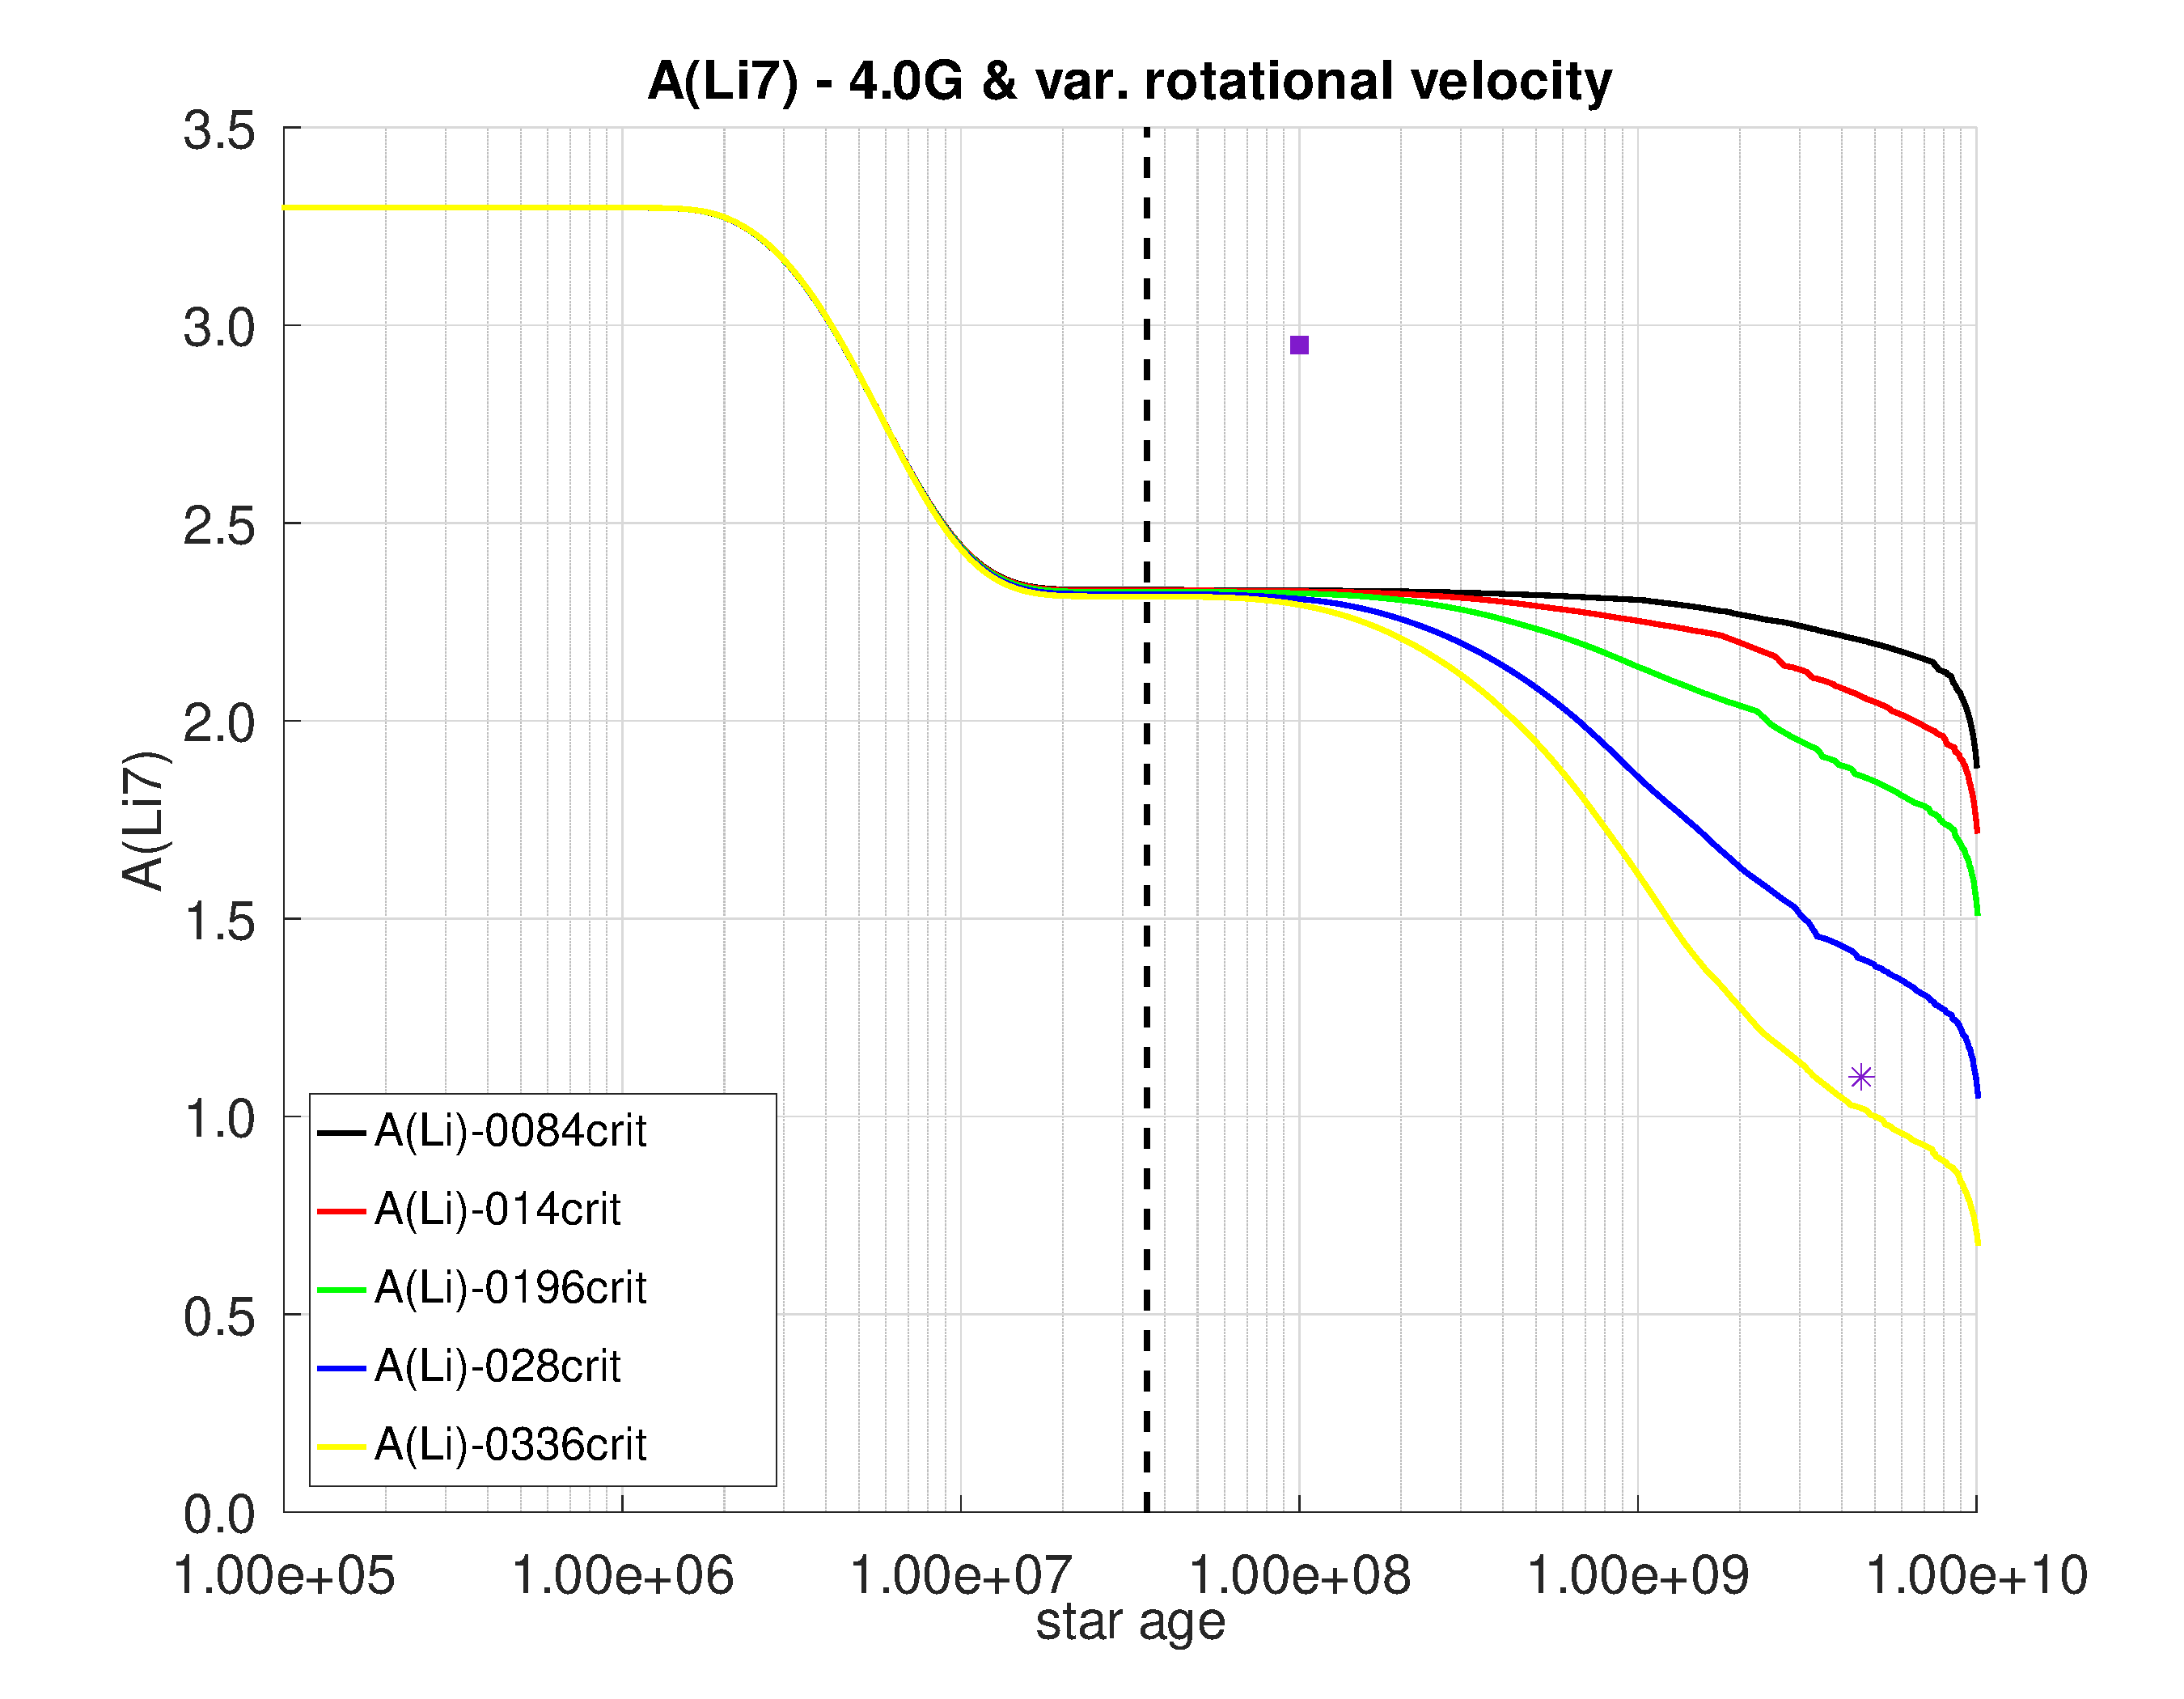
\includegraphics[width=0.7\textwidth]{img/paper1/li_var_vel_4_0g.pdf}
	\caption{Evolución de la abundancia superficial del \isotope[7]{Li} respecto al \isotope[1]{H}, en función del tiempo para varios modelos de 1 $\msun$. Los modelos incluyen un campo magnético con una intensidad de 4G y rotación PMS con $\oomegac$ entre 0,0084 y 0,0336, respectivamente. La estrella púrpura y el cuadrado son la abundancia superficial de Li para el Sol actual \cite{Asplund2009} y el cúmulo de las Pléyades \cite{Sestito2005} respectivamente. La línea vertical discontinua hace referencia a la ZAMS.}
	\label{fig:li_var_vel_4_0g}
\end{figure}

El efecto de la rutina MB puede apreciarse aún más claramente en las Figuras~\ref{fig:rot_vel_4g}, \ref{fig:rot_vel_4g_z1} \& Apéndices \footnote{Los apéndices comprenden una serie de cuadrículas en función del tiempo y para varios modelos de 1 $\msun$ en los que se muestra, por un lado, la evolución de la abundancia superficial del \isotope[7]{Li} respecto al \isotope[1]{H} tanto para intensidades de campo magnético variables como para velocidades angulares y, por otro, la evolución de la velocidad de rotación superficial.}. En estas figuras representamos los perfiles de rotación para la superficie de las estrellas y para el fondo de la envoltura convectiva. Son modelos de 1 $\msun$ inicializados con diferentes velocidades de rotación y considerando la influencia del MB. De forma similar a los perfiles de evolución de $A(\isotope[7]{Li})$ comentados en el párrafo anterior, el efecto de la rutina se hizo visible una vez alcanzada la ZAMS. Si comparamos la evolución de las curvas aquí presentadas con las de la Figura \ref{fig:rot_vel_0g} vemos como la estrella, en lugar de seguir aumentando $\Omega$, comenzó a ralentizarse tras haber alcanzado su máximo en el paso por la ZAMS. Nótese que en este punto las velocidades angulares en la superficie de la estrella y en la ZAMS alcanzaron su máxima diferencia. Por otro lado, el efecto MB hizo que las velocidades angulares entre ambas zonas de la estrella disminuyeran hasta que, para una edad cercana a la del Sol (ver Figura \ref{fig:rot_vel_4g_z1}), la estrella prácticamente rotaba como un sólido rígido. Estos resultados también eran coherentes con los obtenidos por \cite{Eggenberger2010} en cuanto al efecto del campo magnético, en particular su influencia en la pérdida de momento angular, sobre la velocidad de rotación de la estrella.\par

De forma similar, también observamos que los modelos con menor velocidad angular generalmente acababan mostrando valores más altos para la abundancia de Li en la superficie (ver Figuras~ \ref{fig:li_var_vel_4_0g}, \ref{fig:grid_li_var_vel} y \ref{fig:grid_li_var_g}). En ninguno de esos casos obtuvimos valores de Li en la superficie superiores a los mostrados por el modelo sin rotación.\par


\begin{figure}
    \centering
    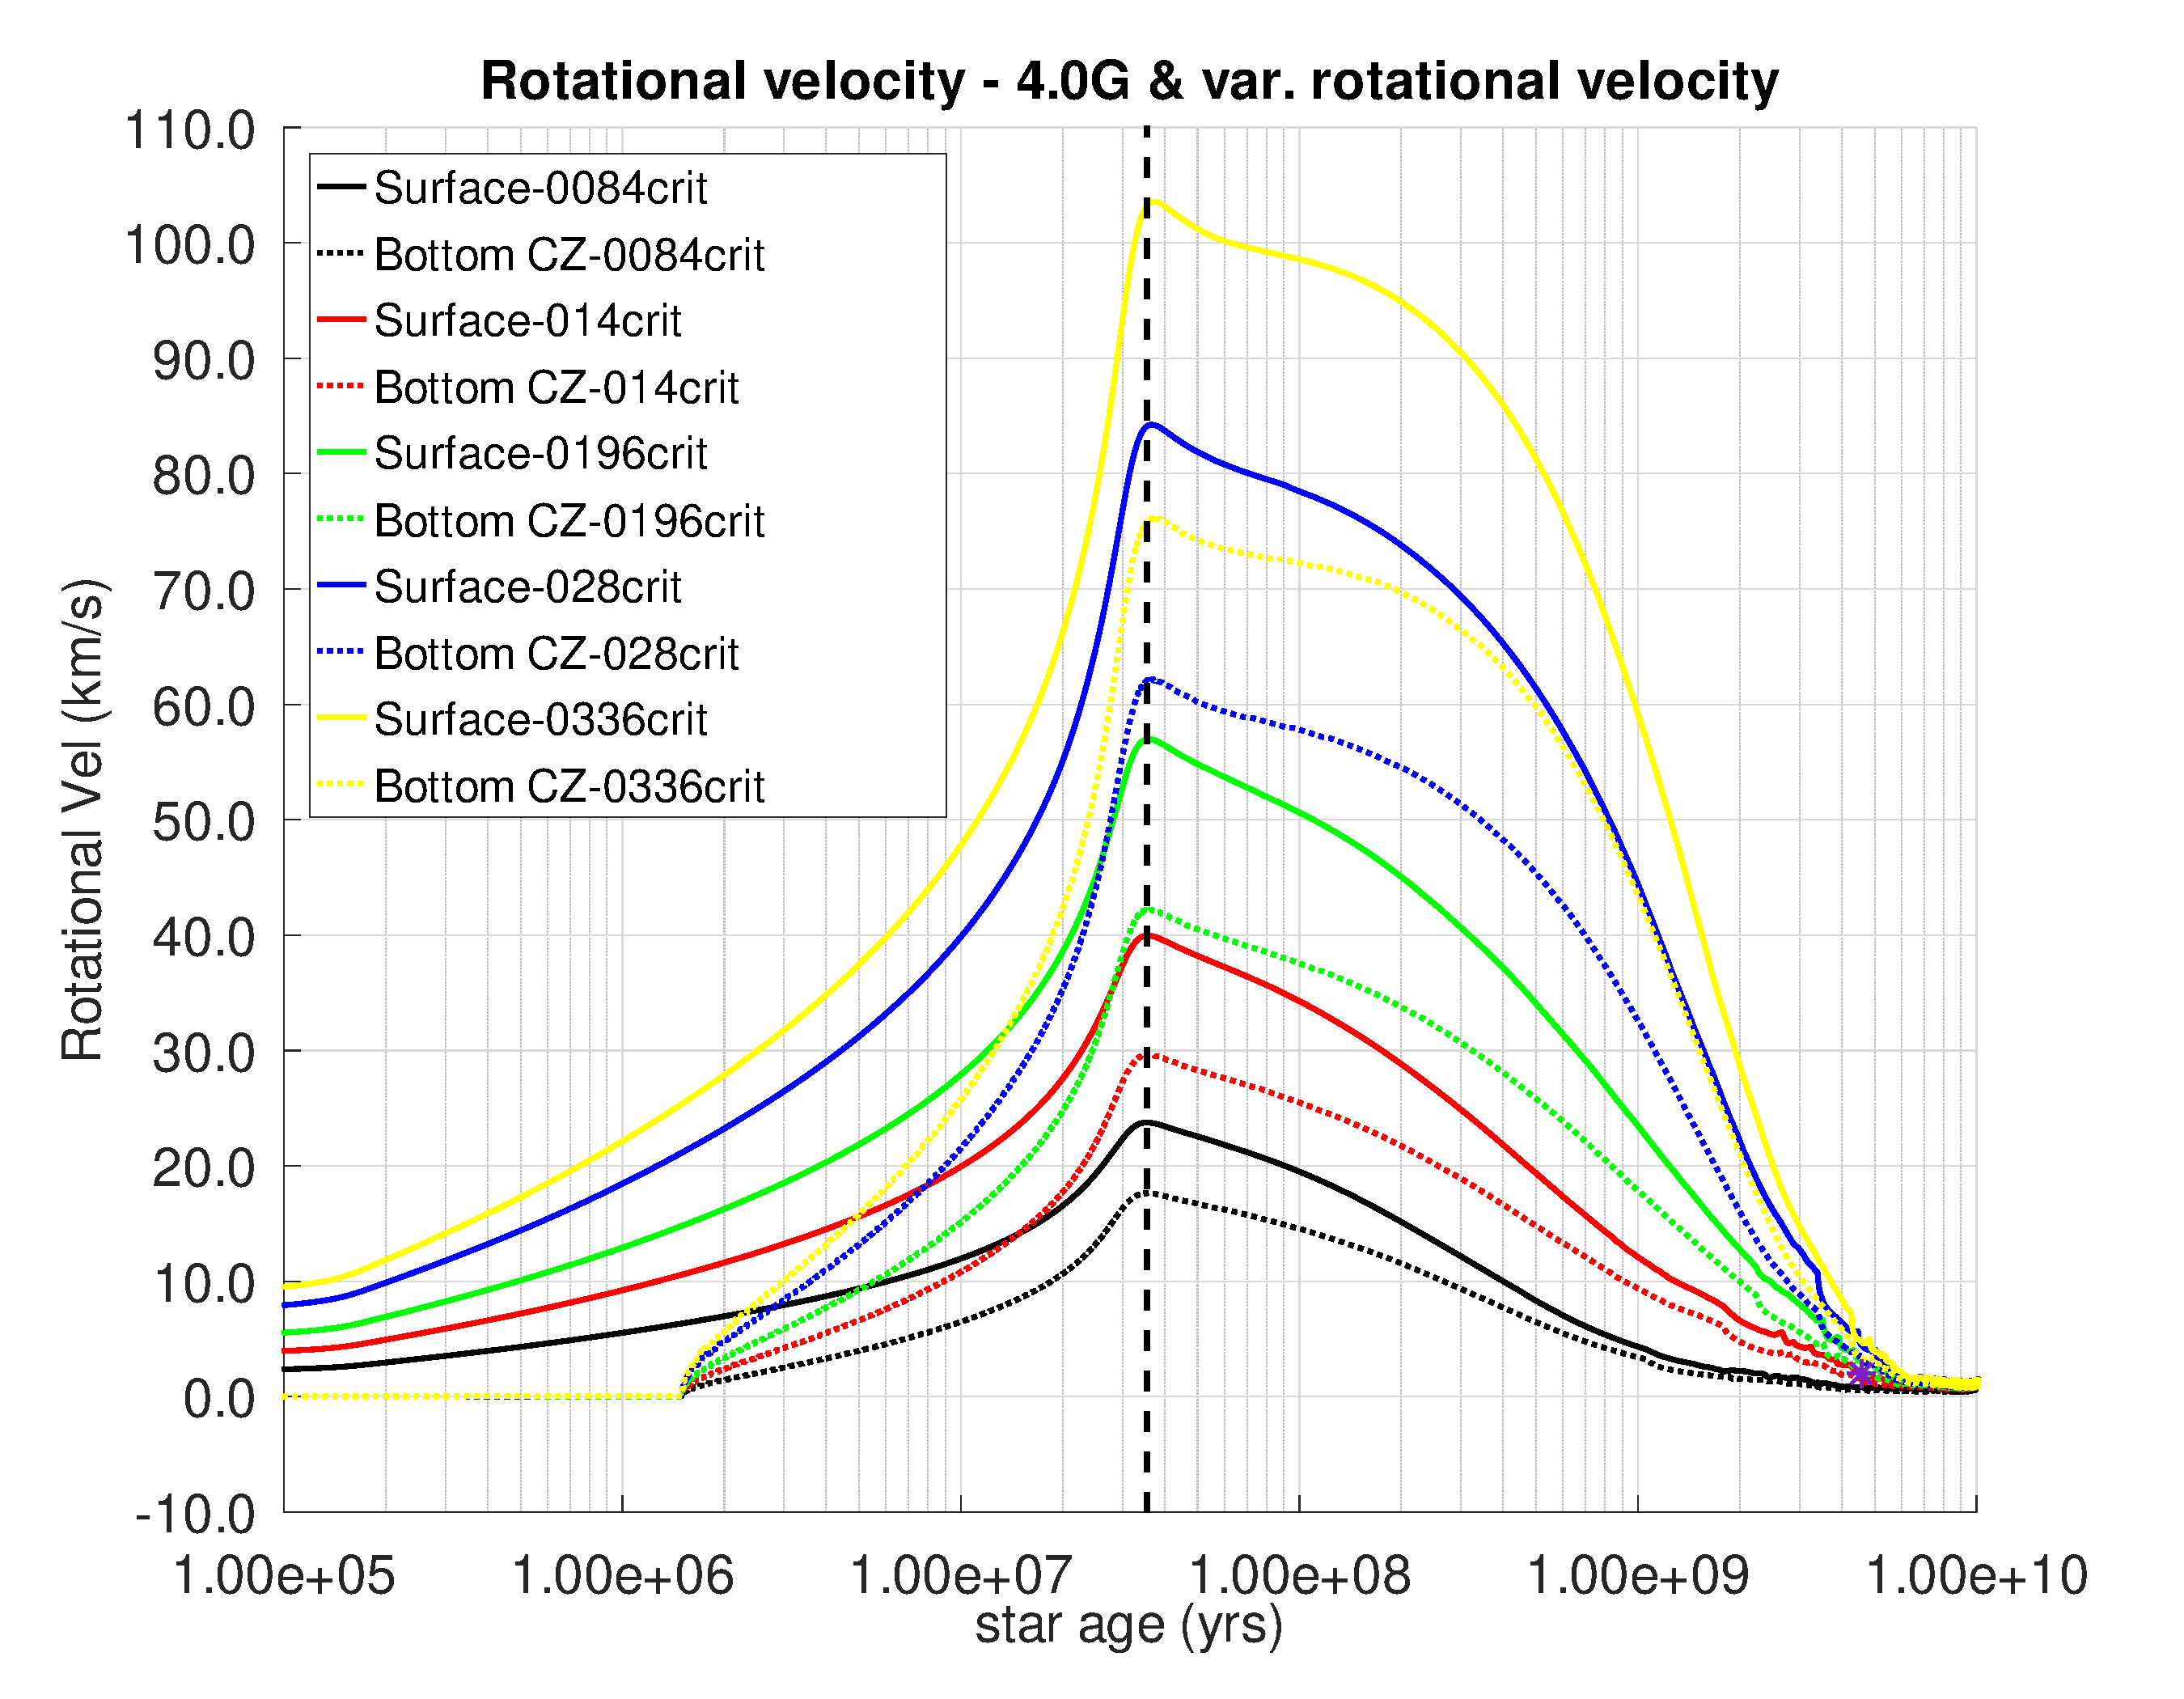
\includegraphics[width=0.7\textwidth]{img/paper1/rot_vel_var_vel_4_0g.pdf}
	\caption{La evolución de la velocidad de rotación de la superficie, en función del tiempo para varios modelos de 1 $\msun$. Los modelos incluyen un campo magnético con una intensidad de 4\,G, rotación PMS con $\oomegac$ entre 0,0084 y 0,0336, respectivamente y MB. La estrella púrpura es la velocidad angular superficial para el Sol actual \cite{Gill2012}. La línea vertical discontinua hace referencia a la ZAMS.}
	\label{fig:rot_vel_4g}
\end{figure}

\begin{figure}
    \centering
    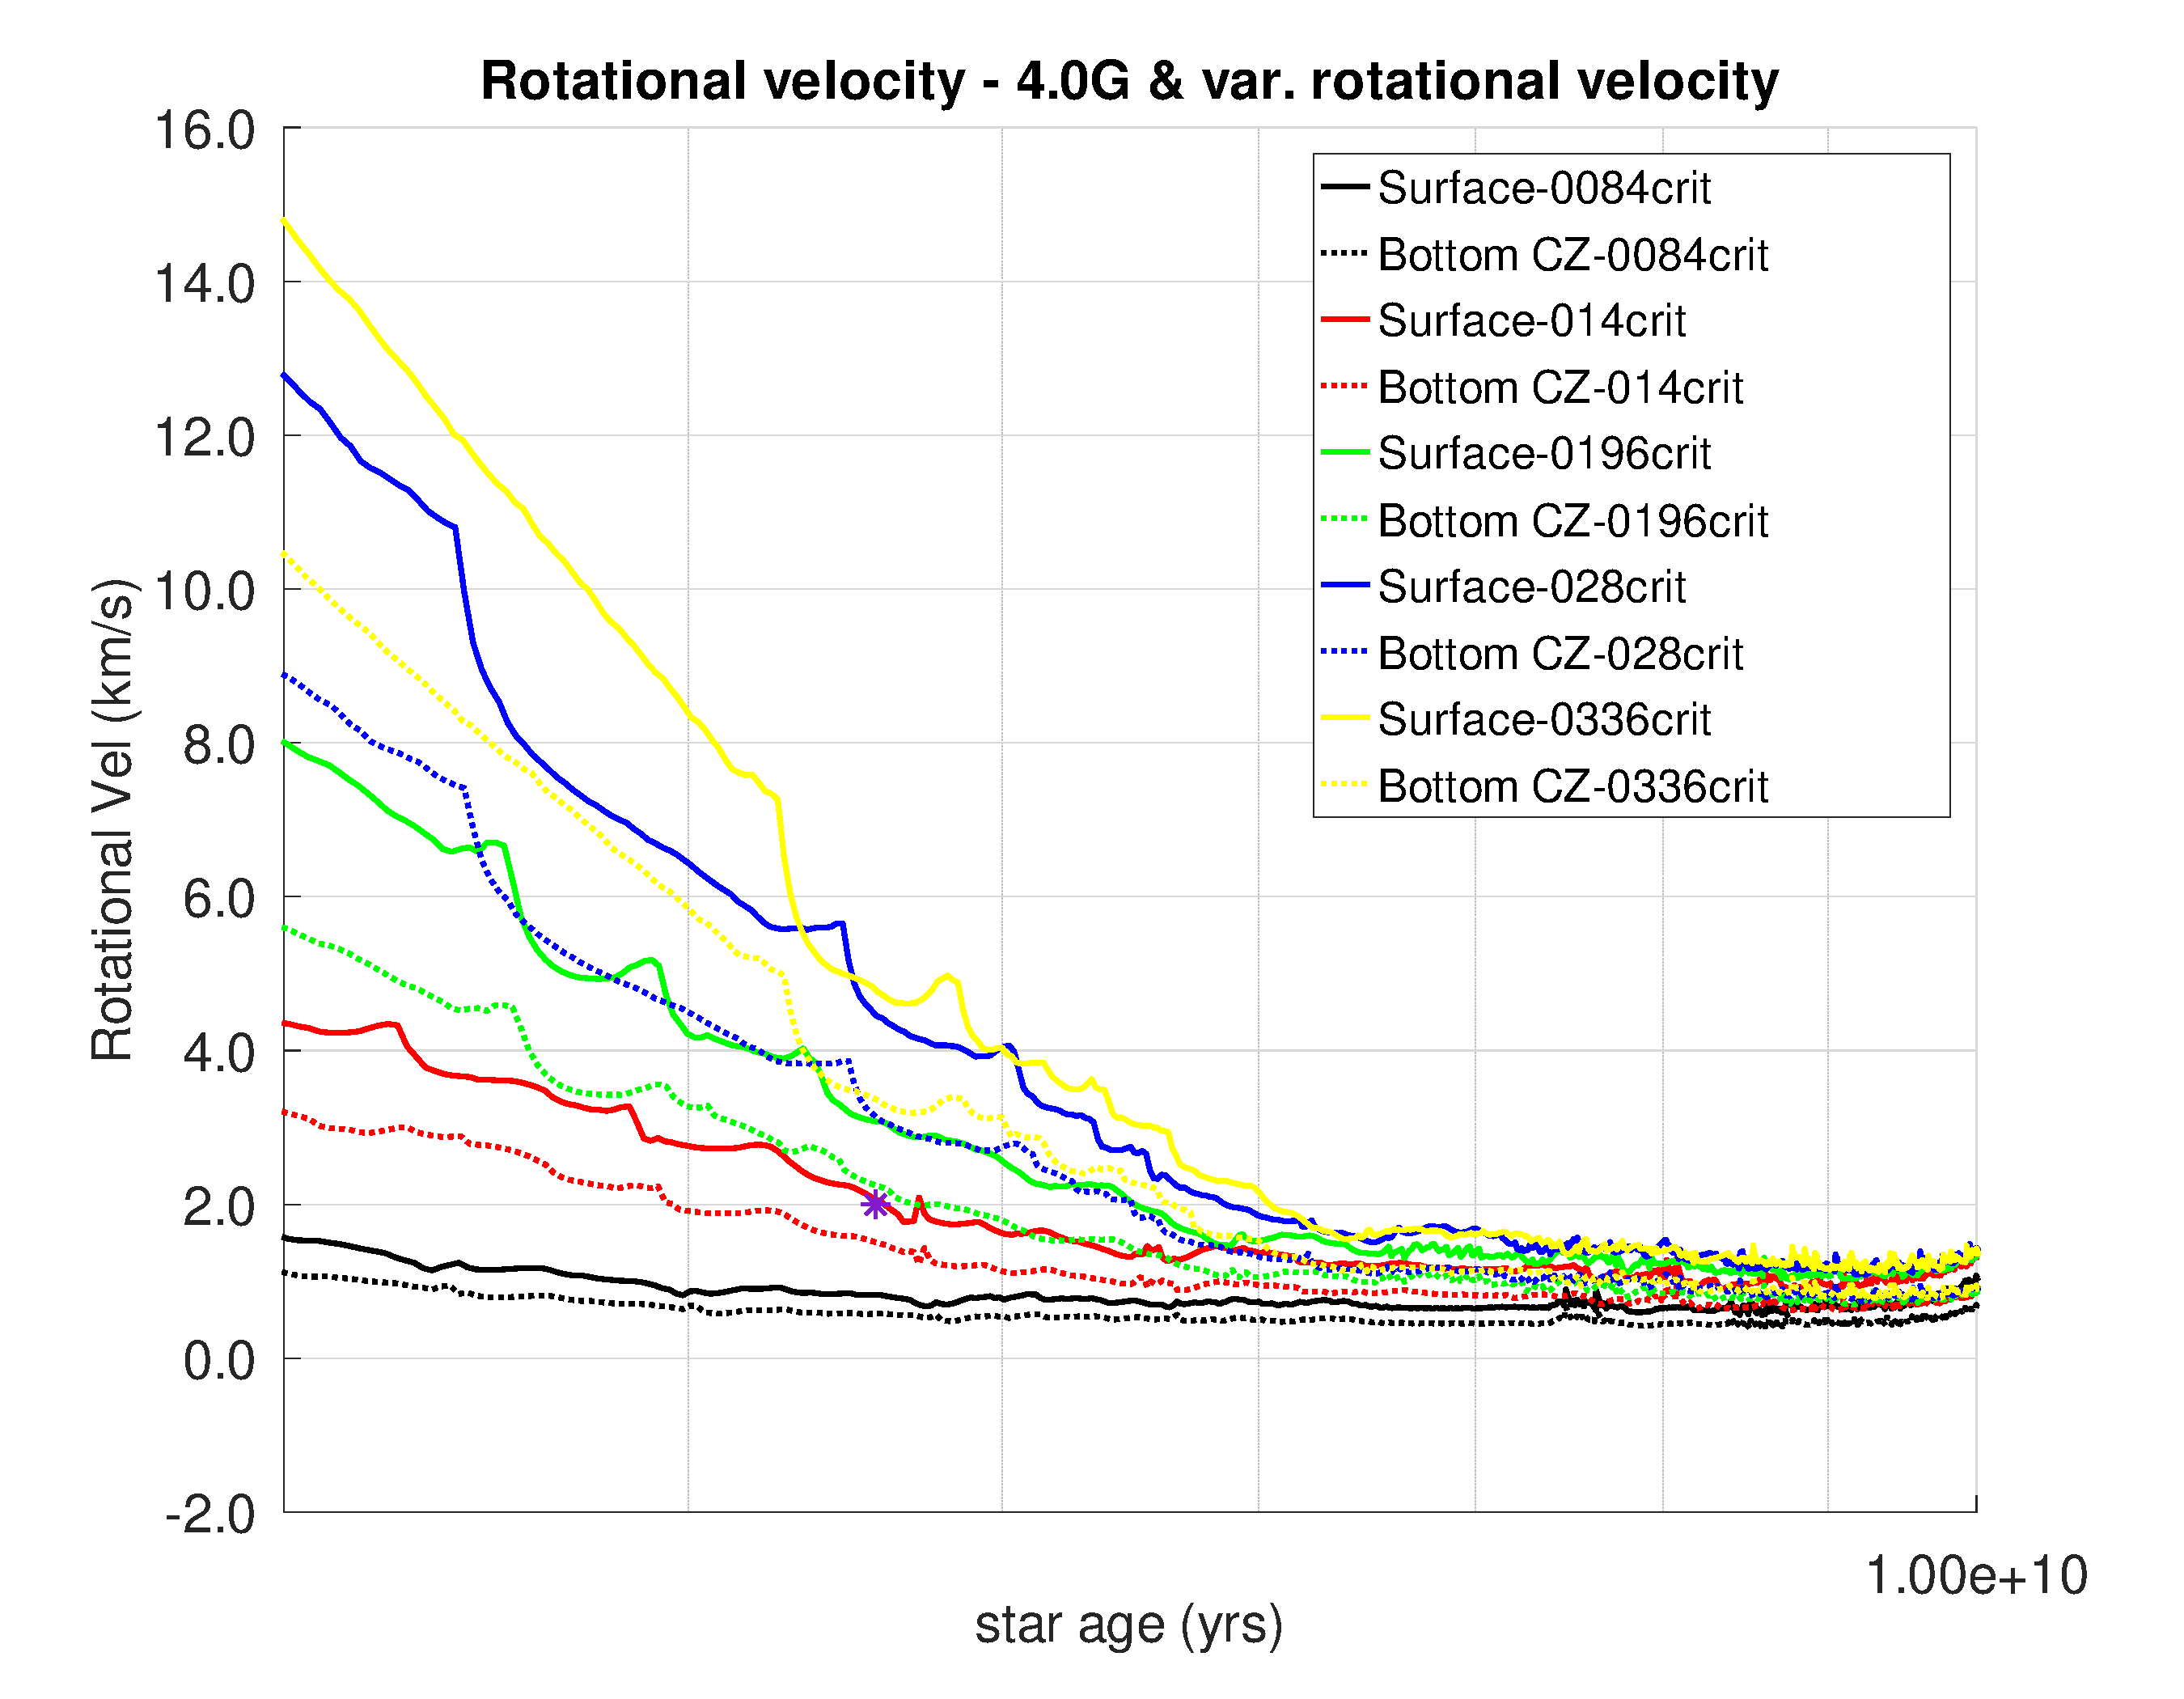
\includegraphics[width=0.7\textwidth]{img/paper1/rot_vel_var_vel_4_0g_z1.pdf}
	\caption{Similar a la Figura \ref{fig:rot_vel_4g} pero ahora mostrando en detalle la velocidad de rotación de la superficie a medida que la estrella se aproxima a TAMS.}
	\label{fig:rot_vel_4g_z1}
\end{figure}

El MB también dejó su huella en el diagrama HR afectando significativamente al $\teff$ de la estrella. Para visualizar este efecto tomamos como referencia la Figura \ref{hr_vc_0336_var_g_z1} en la que todos los modelos se iniciaron con el mismo valor $\oomegac=0,0336$ pero la intensidad del campo magnético simulado fue diferente. Obsérvese que los modelos con MB produjeron estrellas más calientes debido a su influencia. La menor velocidad con la que giraba la estrella debido al efecto MB provocó el aumento del $\teff$, siendo esta diferencia de prácticamente 95K entre los modelos simulados con 0.0G y 5.0G respectivamente para $log(\llsun)=0$.

\begin{figure}
    \centering
    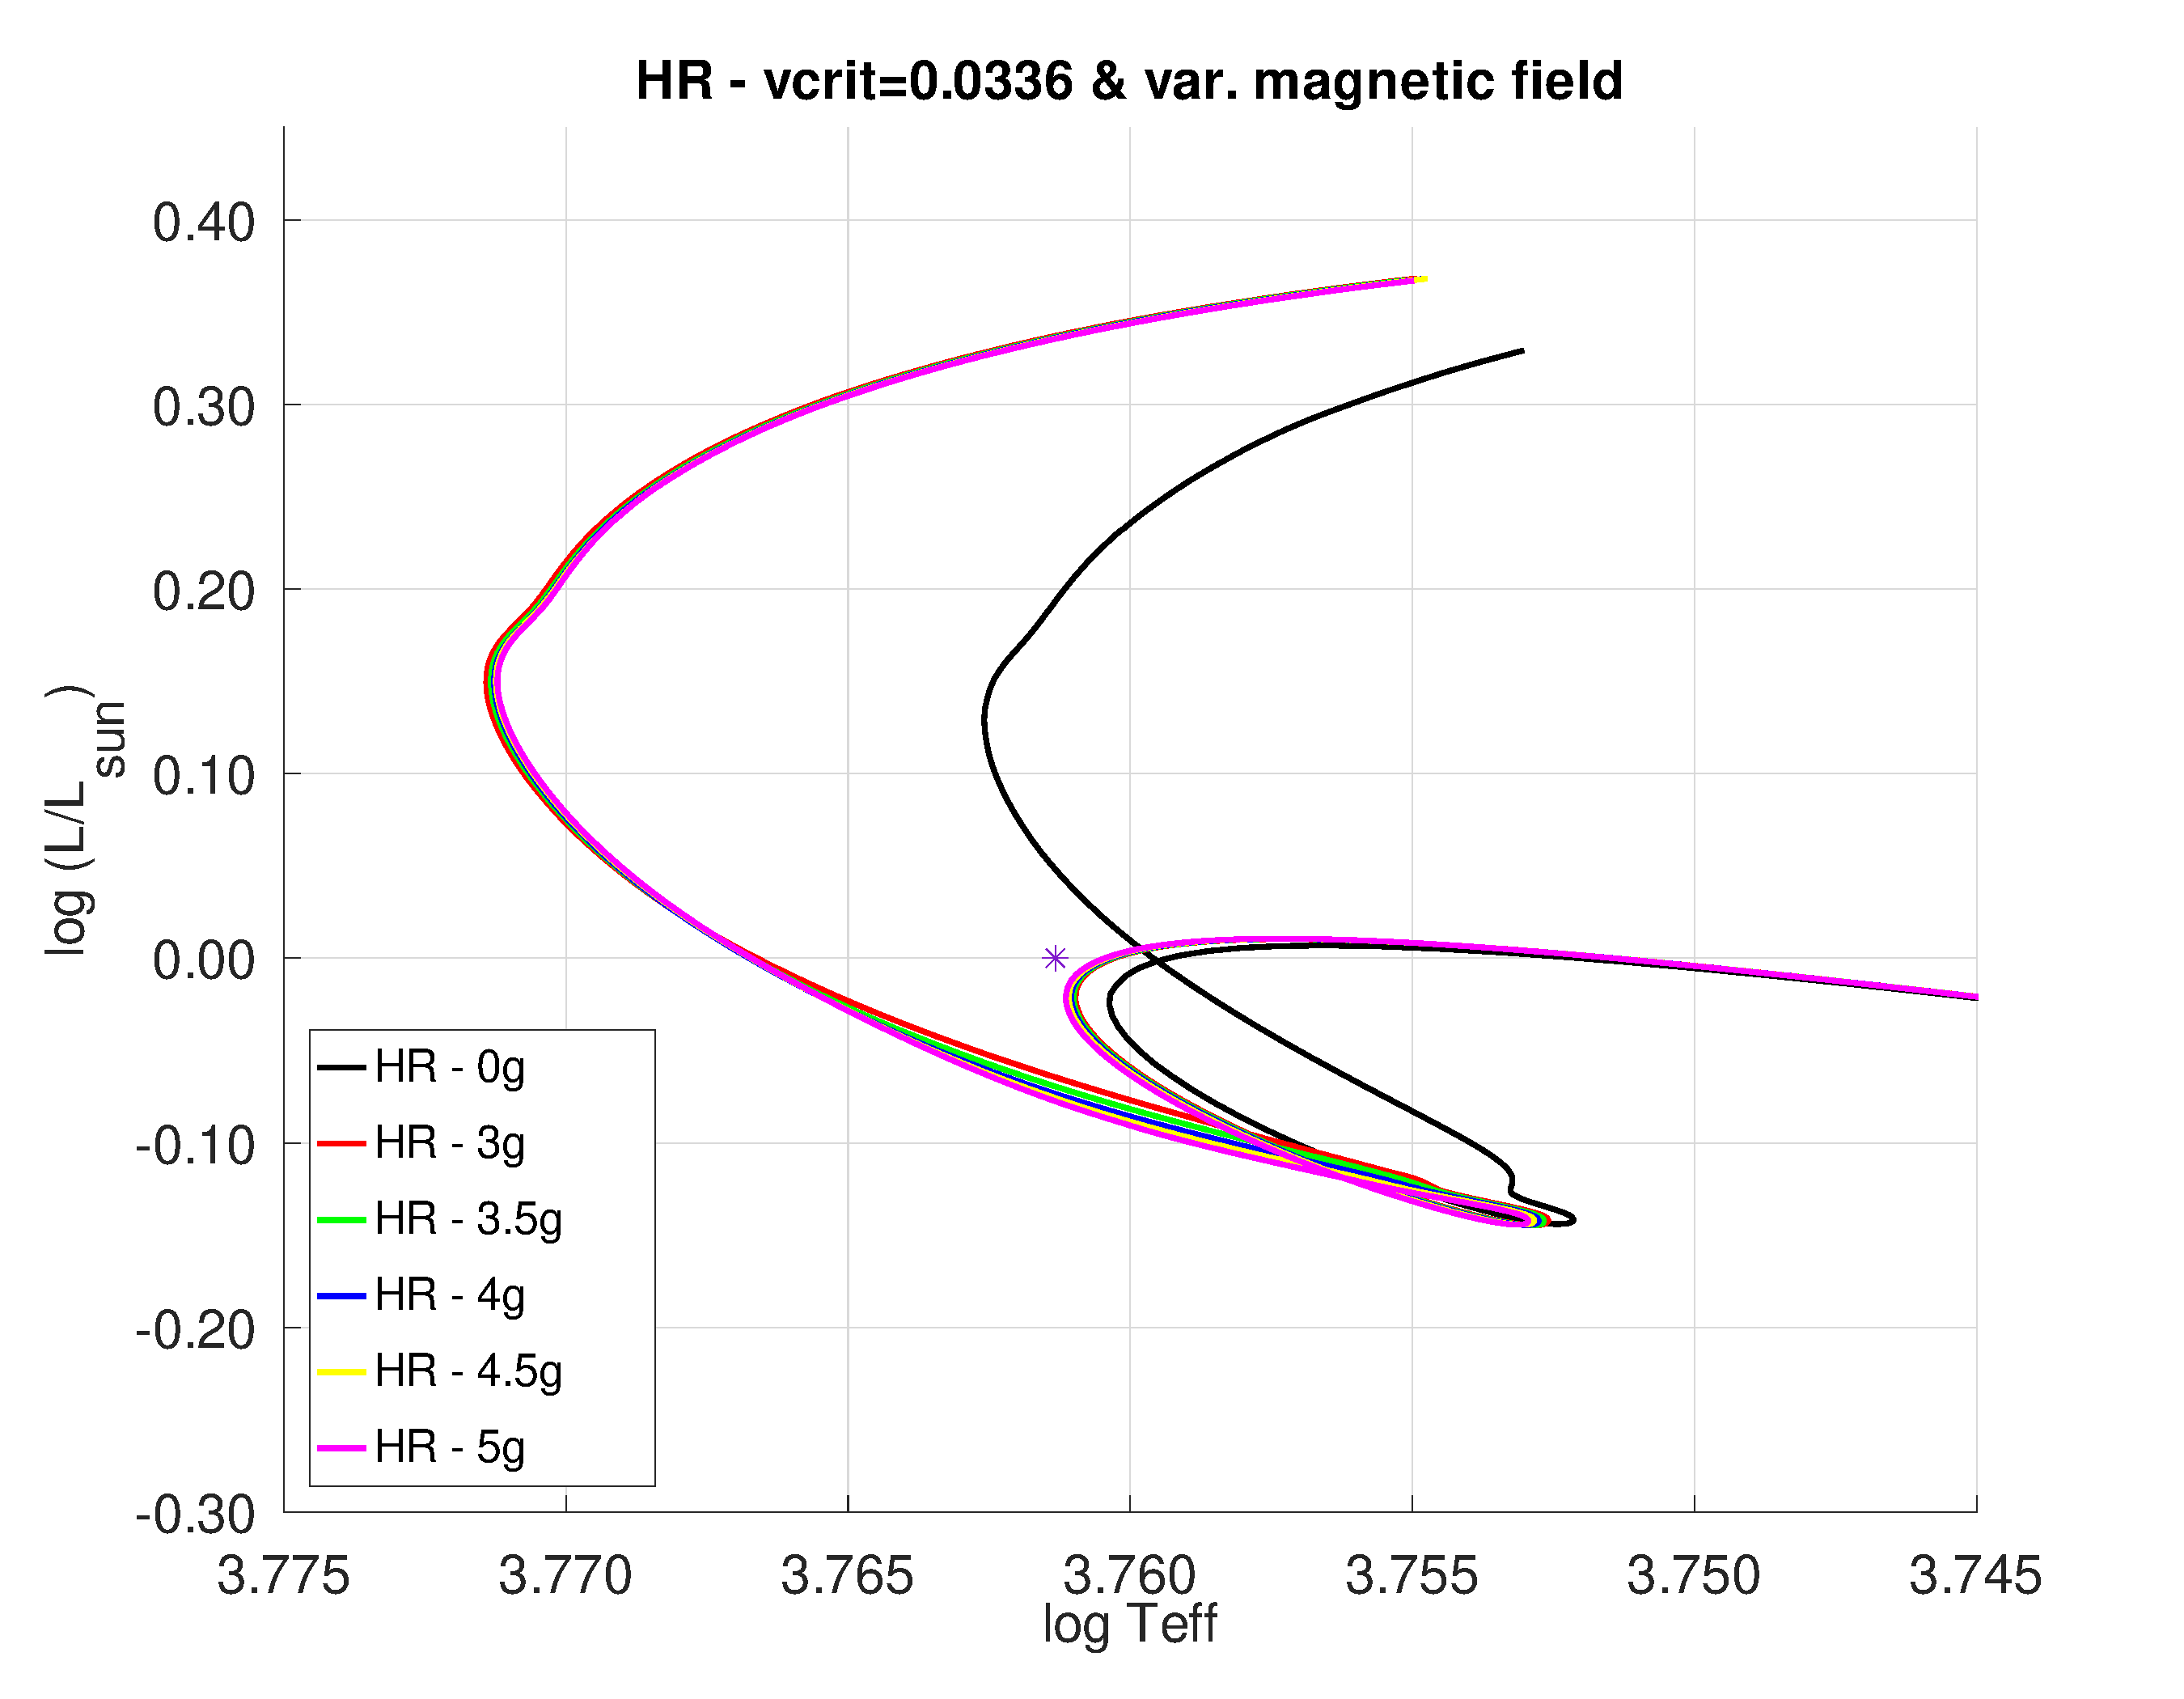
\includegraphics[width=0.7\textwidth]{img/paper1/hr_vc_0336_var_g_z1.pdf}
	\caption{Similar a la Figura \ref{fig:hr_var_vel_0g} pero ahora mostrando en detalle los efectos del frenado magnético en las trayectorias evolutivas para diferentes intensidades de campo magnético y $\oomegac=0.0336$. La presencia de un campo magnético produce estrellas más calientes debido a la influencia del frenado magnético en la velocidad de rotación de la estrella.}
	\label{hr_vc_0336_var_g_z1}
\end{figure}

Como se describe en la sección \ref{sec_mesh}, la rutina MB distribuyó la cantidad total de AML calculada según la Ec.~\ref{eq:k_jdot} entre las distintas capas que componían la CZ. En la Figura \ref{fig:cz_vc_028_var_b} podemos observar la evolución de la CZ más externa normalizada con respecto al radio de la estrella para varios modelos de 1 $\msun$. Todos los modelos se inicializaron con $\oomegac=0.0336$ e intensidades de campo magnético que variaban entre 0.0G y 5.0G. De acuerdo con los modelos establecidos de evolución estelar, en una estrella de tipo solar la CZ cubre prácticamente toda ella durante gran parte del PMS. A medida que se aproxima a la ZAMS, la CZ va disminuyendo como consecuencia de la aparición de un núcleo radiativo y mantiene un radio aproximadamente constante hasta la etapa final de la MS. En este punto aumenta significativamente como respuesta a la expansión generalizada del radio de la estrella. En cuanto al efecto deL MB sobre el tamaño de la CZ, observamos que a medida que aumentaba la intensidad del campo magnético, el tamaño de la CZ disminuía (véase la figura \ref{fig:cz_vc_028_var_b_z1_new}). El núcleo radiativo se desplazó hacia el exterior para incluir una fracción cada vez mayor de la masa estelar, haciendo que la temperatura en la base de la CZ cayera por debajo de $\tli$. Este efecto fue más evidente durante la MS. La disminución del tamaño de la CZ estuvo en consonancia con el hecho de que se destruyera menos Li haciendo que menos material estelar alcanzara zonas con temperaturas superiores a $\tli$.\par

\begin{figure}
    \centering
    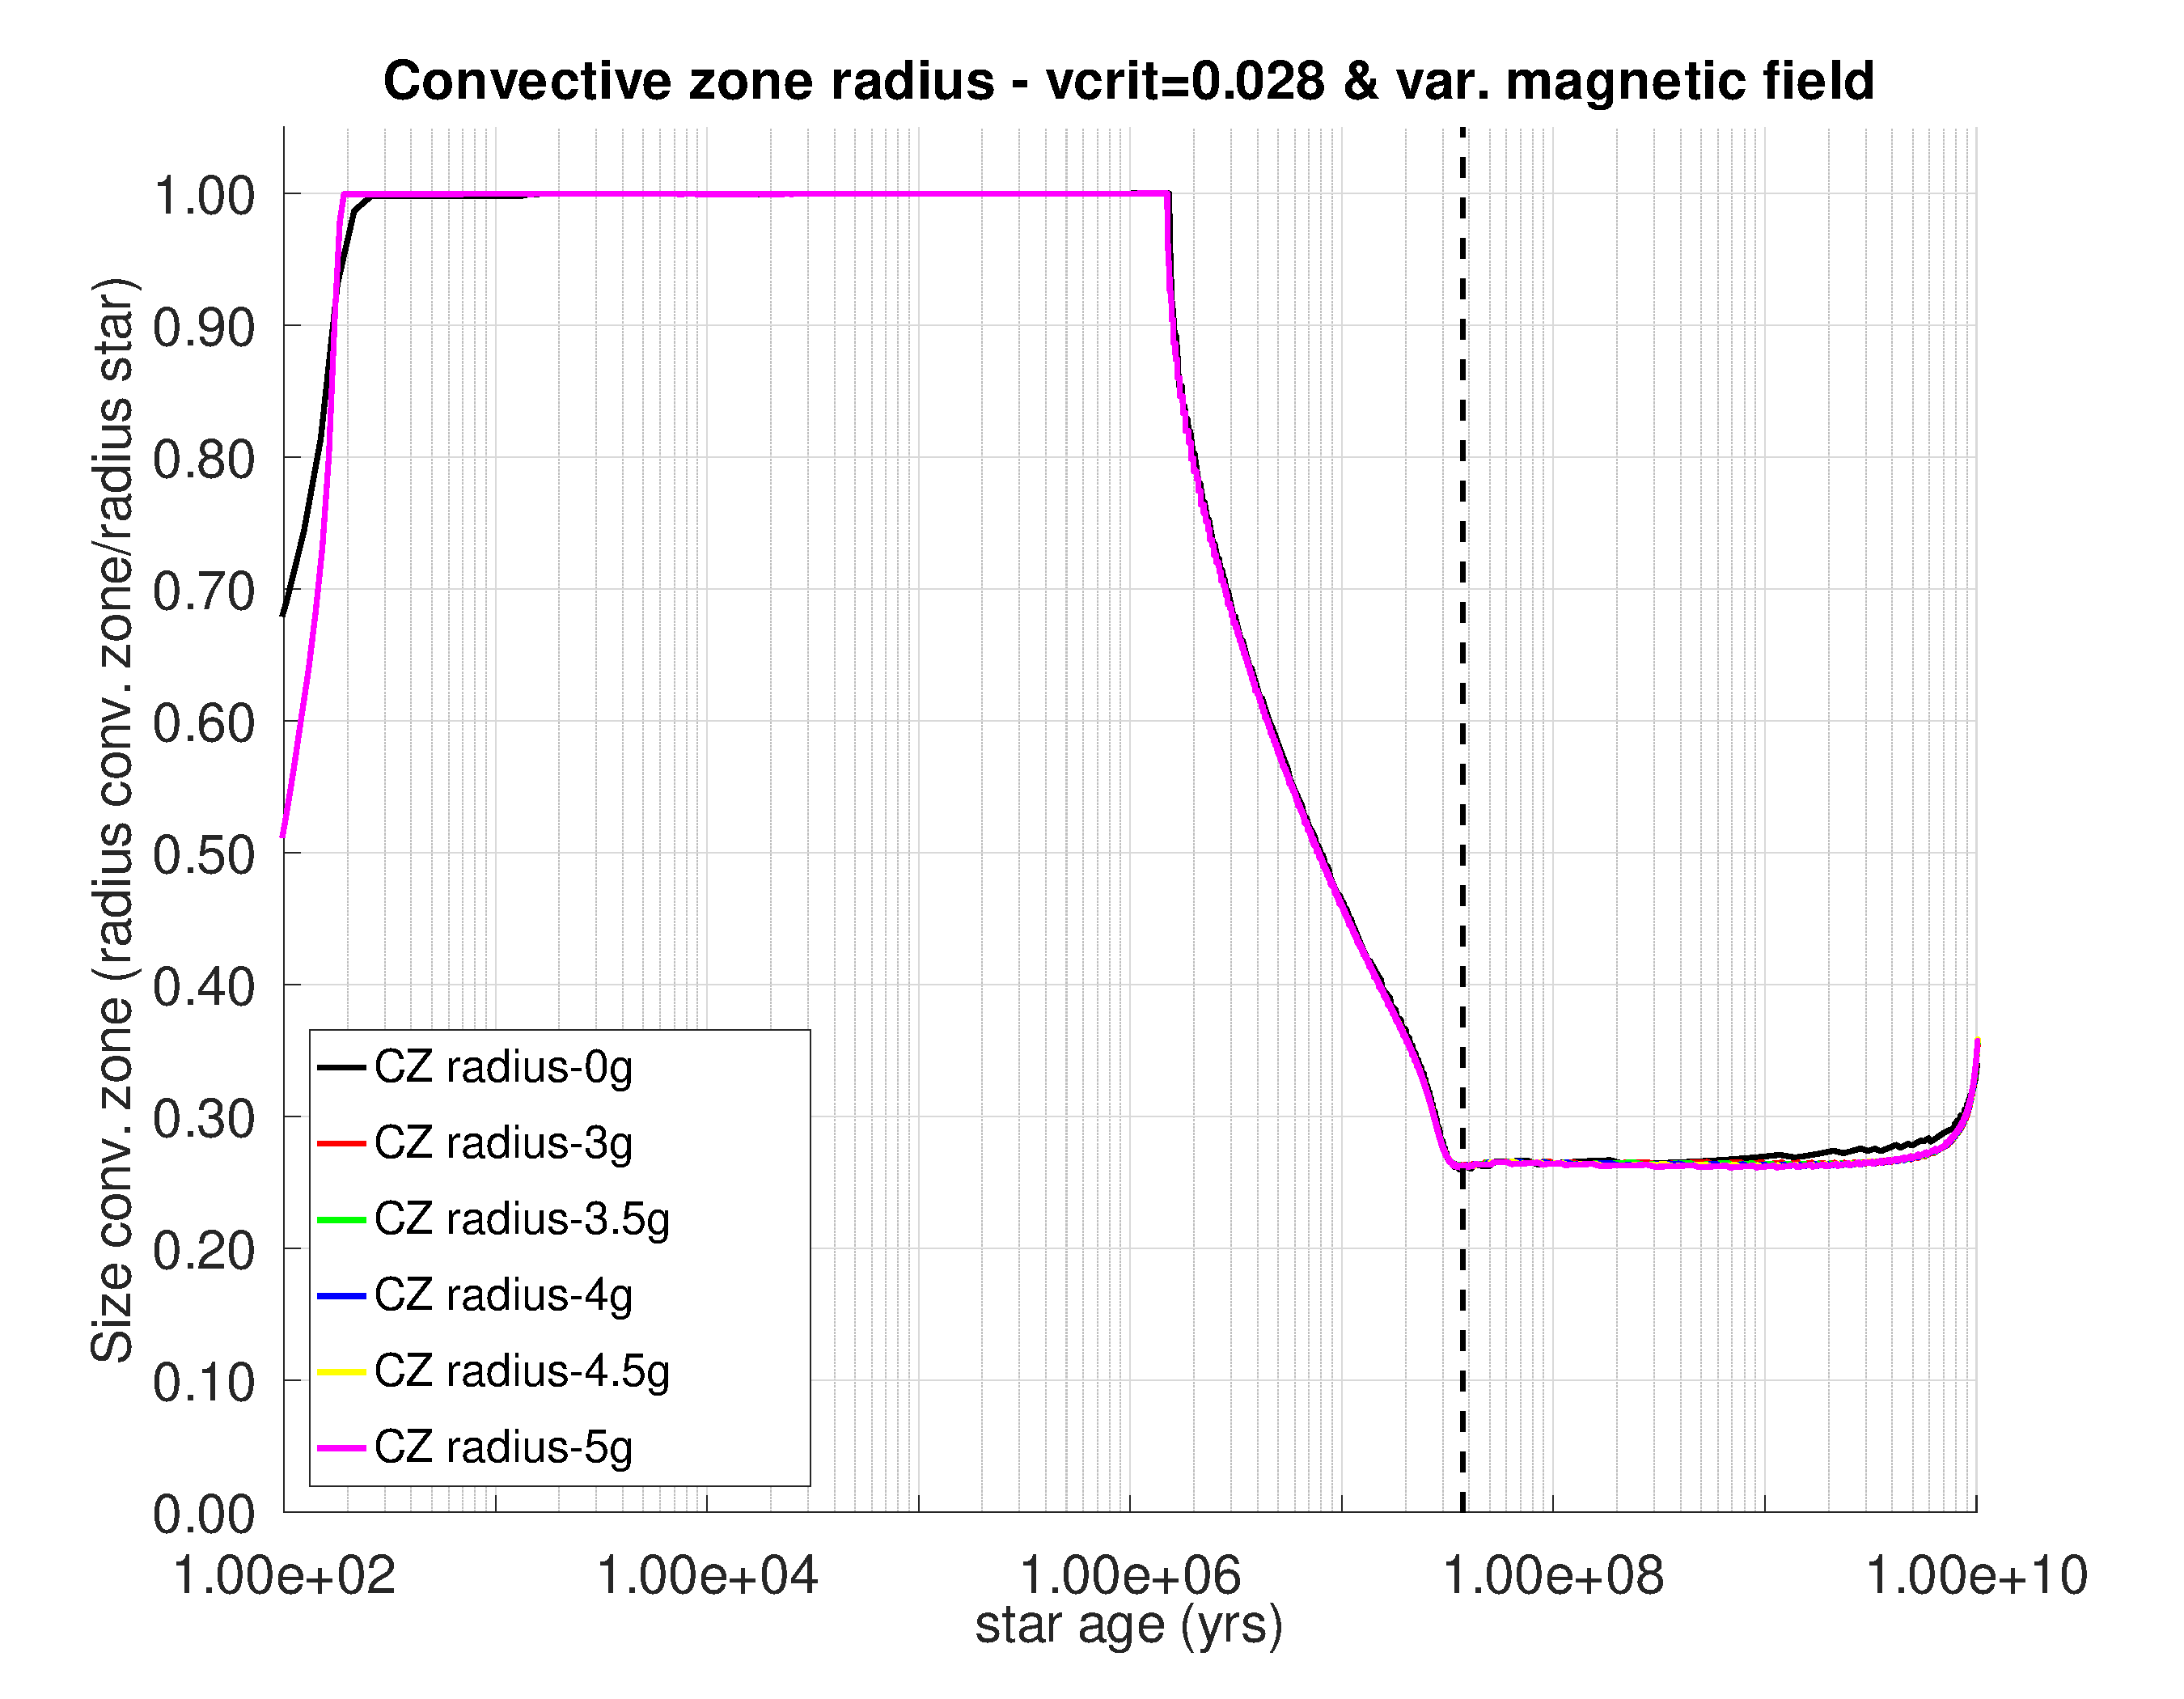
\includegraphics[width=0.7\textwidth]{img/paper1/cz_vc_028_var_g.pdf}
	\caption{Evolución del tamaño de la zona convectiva en función del tiempo para varios modelos de 1 $\msun$. Todos los modelos se inicializaron con $\oomegac=0.0336$ y las intensidades de campo magnético varían entre 0.0G y 5.0G. La línea vertical discontinua hace referencia a la ZAMS.}
	\label{fig:cz_vc_028_var_b}
\end{figure}

En la Figura \ref{fig:mdot_vc_028_var_b} podemos ver la evolución de $\Dot{M}$ durante PMS y MS para varios modelos de 1 $\msun$. Todos los modelos se inicializaron con $\oomegac=0.0336$ e intensidades de campo magnético que variaban entre 0.0G y 5.0G. En las primeras etapas del PMS fue donde se concentró la mayor pérdida de masa, que fue disminuyendo a medida que se acercaba a la ZAMS. Como la estrella también disminuyó su radio durante la PMS, aumentó $\Omega$ obedeciendo al principio de conservación del AM. Al llegar a la ZAMS, el radio estelar se mantuvo más o menos estable durante gran parte de la MS (excepto en su etapa final, véase la figura \ref{fig:mdot_vc_028_var_b_z1}), pero siguió perdiendo masa mientras aumentaba $\Omega$, aunque de forma menos agresiva si lo comparamos con la PMS. Sin embargo, como consecuencia tanto de la aparición del núcleo radiativo durante el seguimiento de Henyey como de la existencia de una CZ (véase la figura \ref{fig:mb_act_var_vel_vc_028}), se activó la rutina MB, provocando que la velocidad angular de la estrella comenzara a disminuir a lo largo de toda la MS. Cuanto más intenso es el campo magnético, mayor es el efecto de frenado.\par 

\begin{figure}
    \centering
    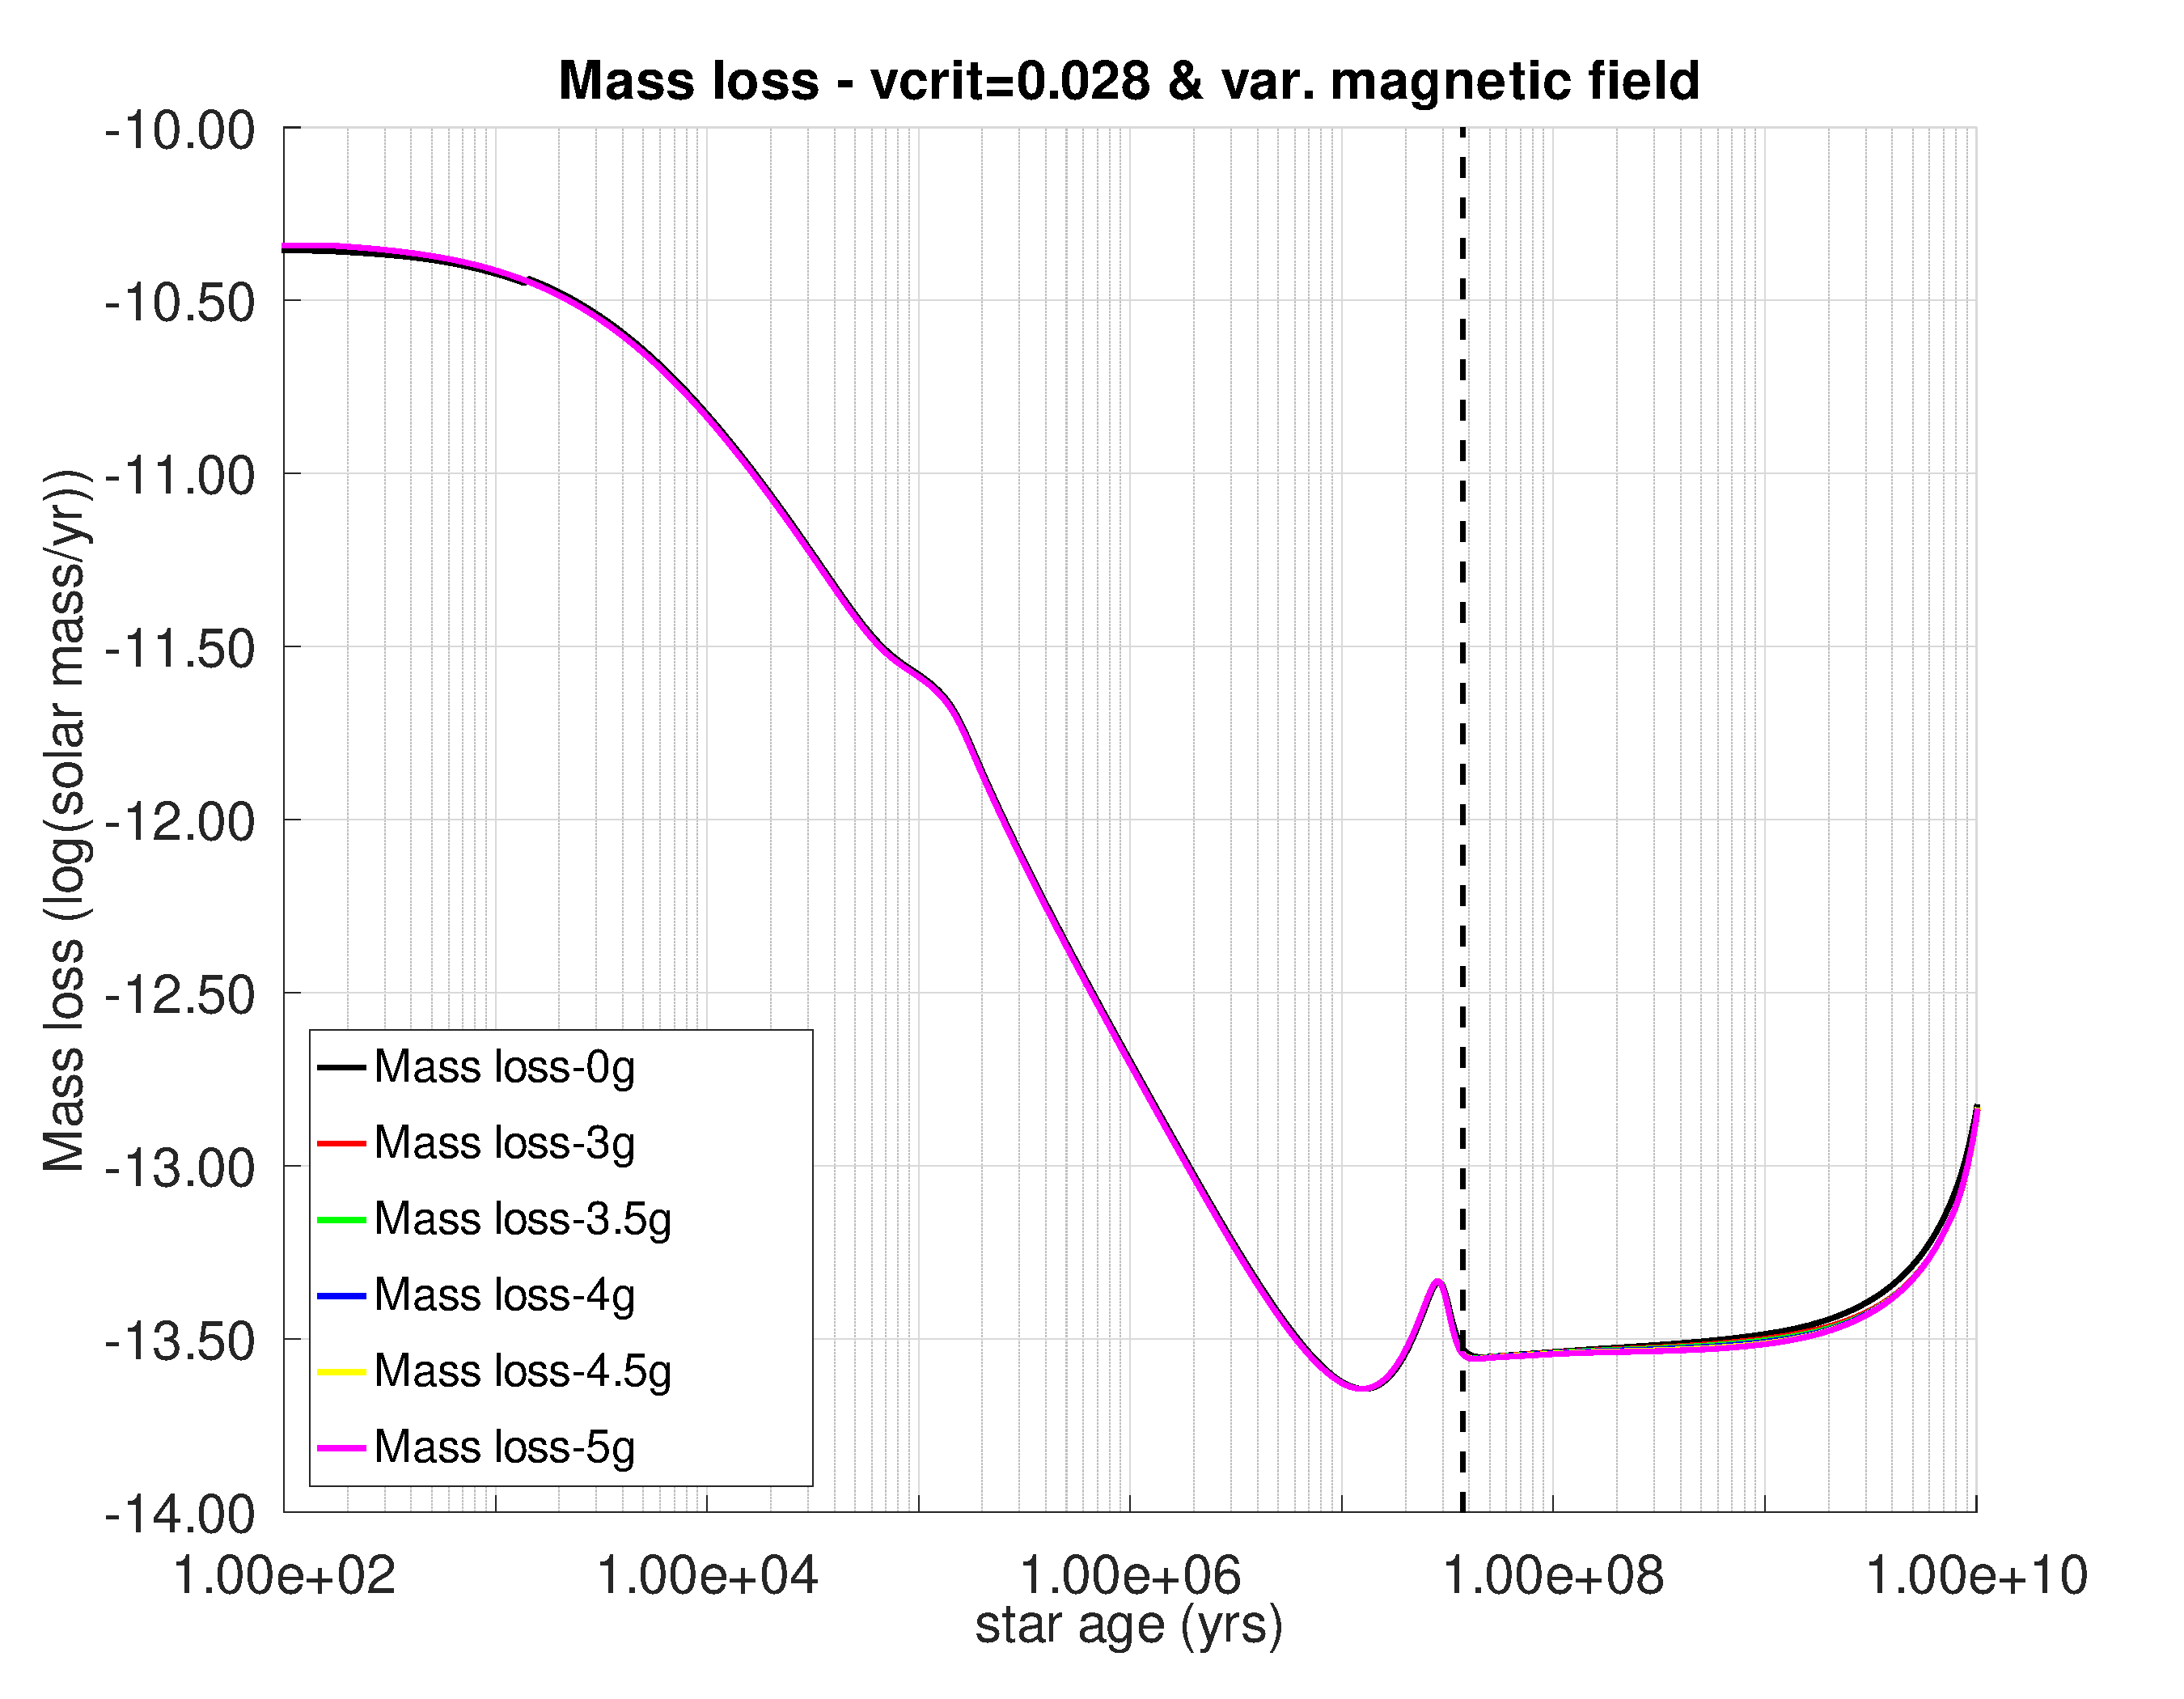
\includegraphics[width=0.7\textwidth]{img/paper1/mdot_vc_028_var_g.pdf}
	\caption{Evolución de la pérdida de masa $\Dot{M}$ en función del tiempo para varios modelos de 1 $\msun$. Los modelos incluyen diferentes intensidades de campo magnético entre 0.0G y 5.0G y rotación PMS con $\oomegac=0.028$. La línea vertical discontinua hace referencia a la ZAMS.}
	\label{fig:mdot_vc_028_var_b}
\end{figure}

\begin{figure}
    \centering
    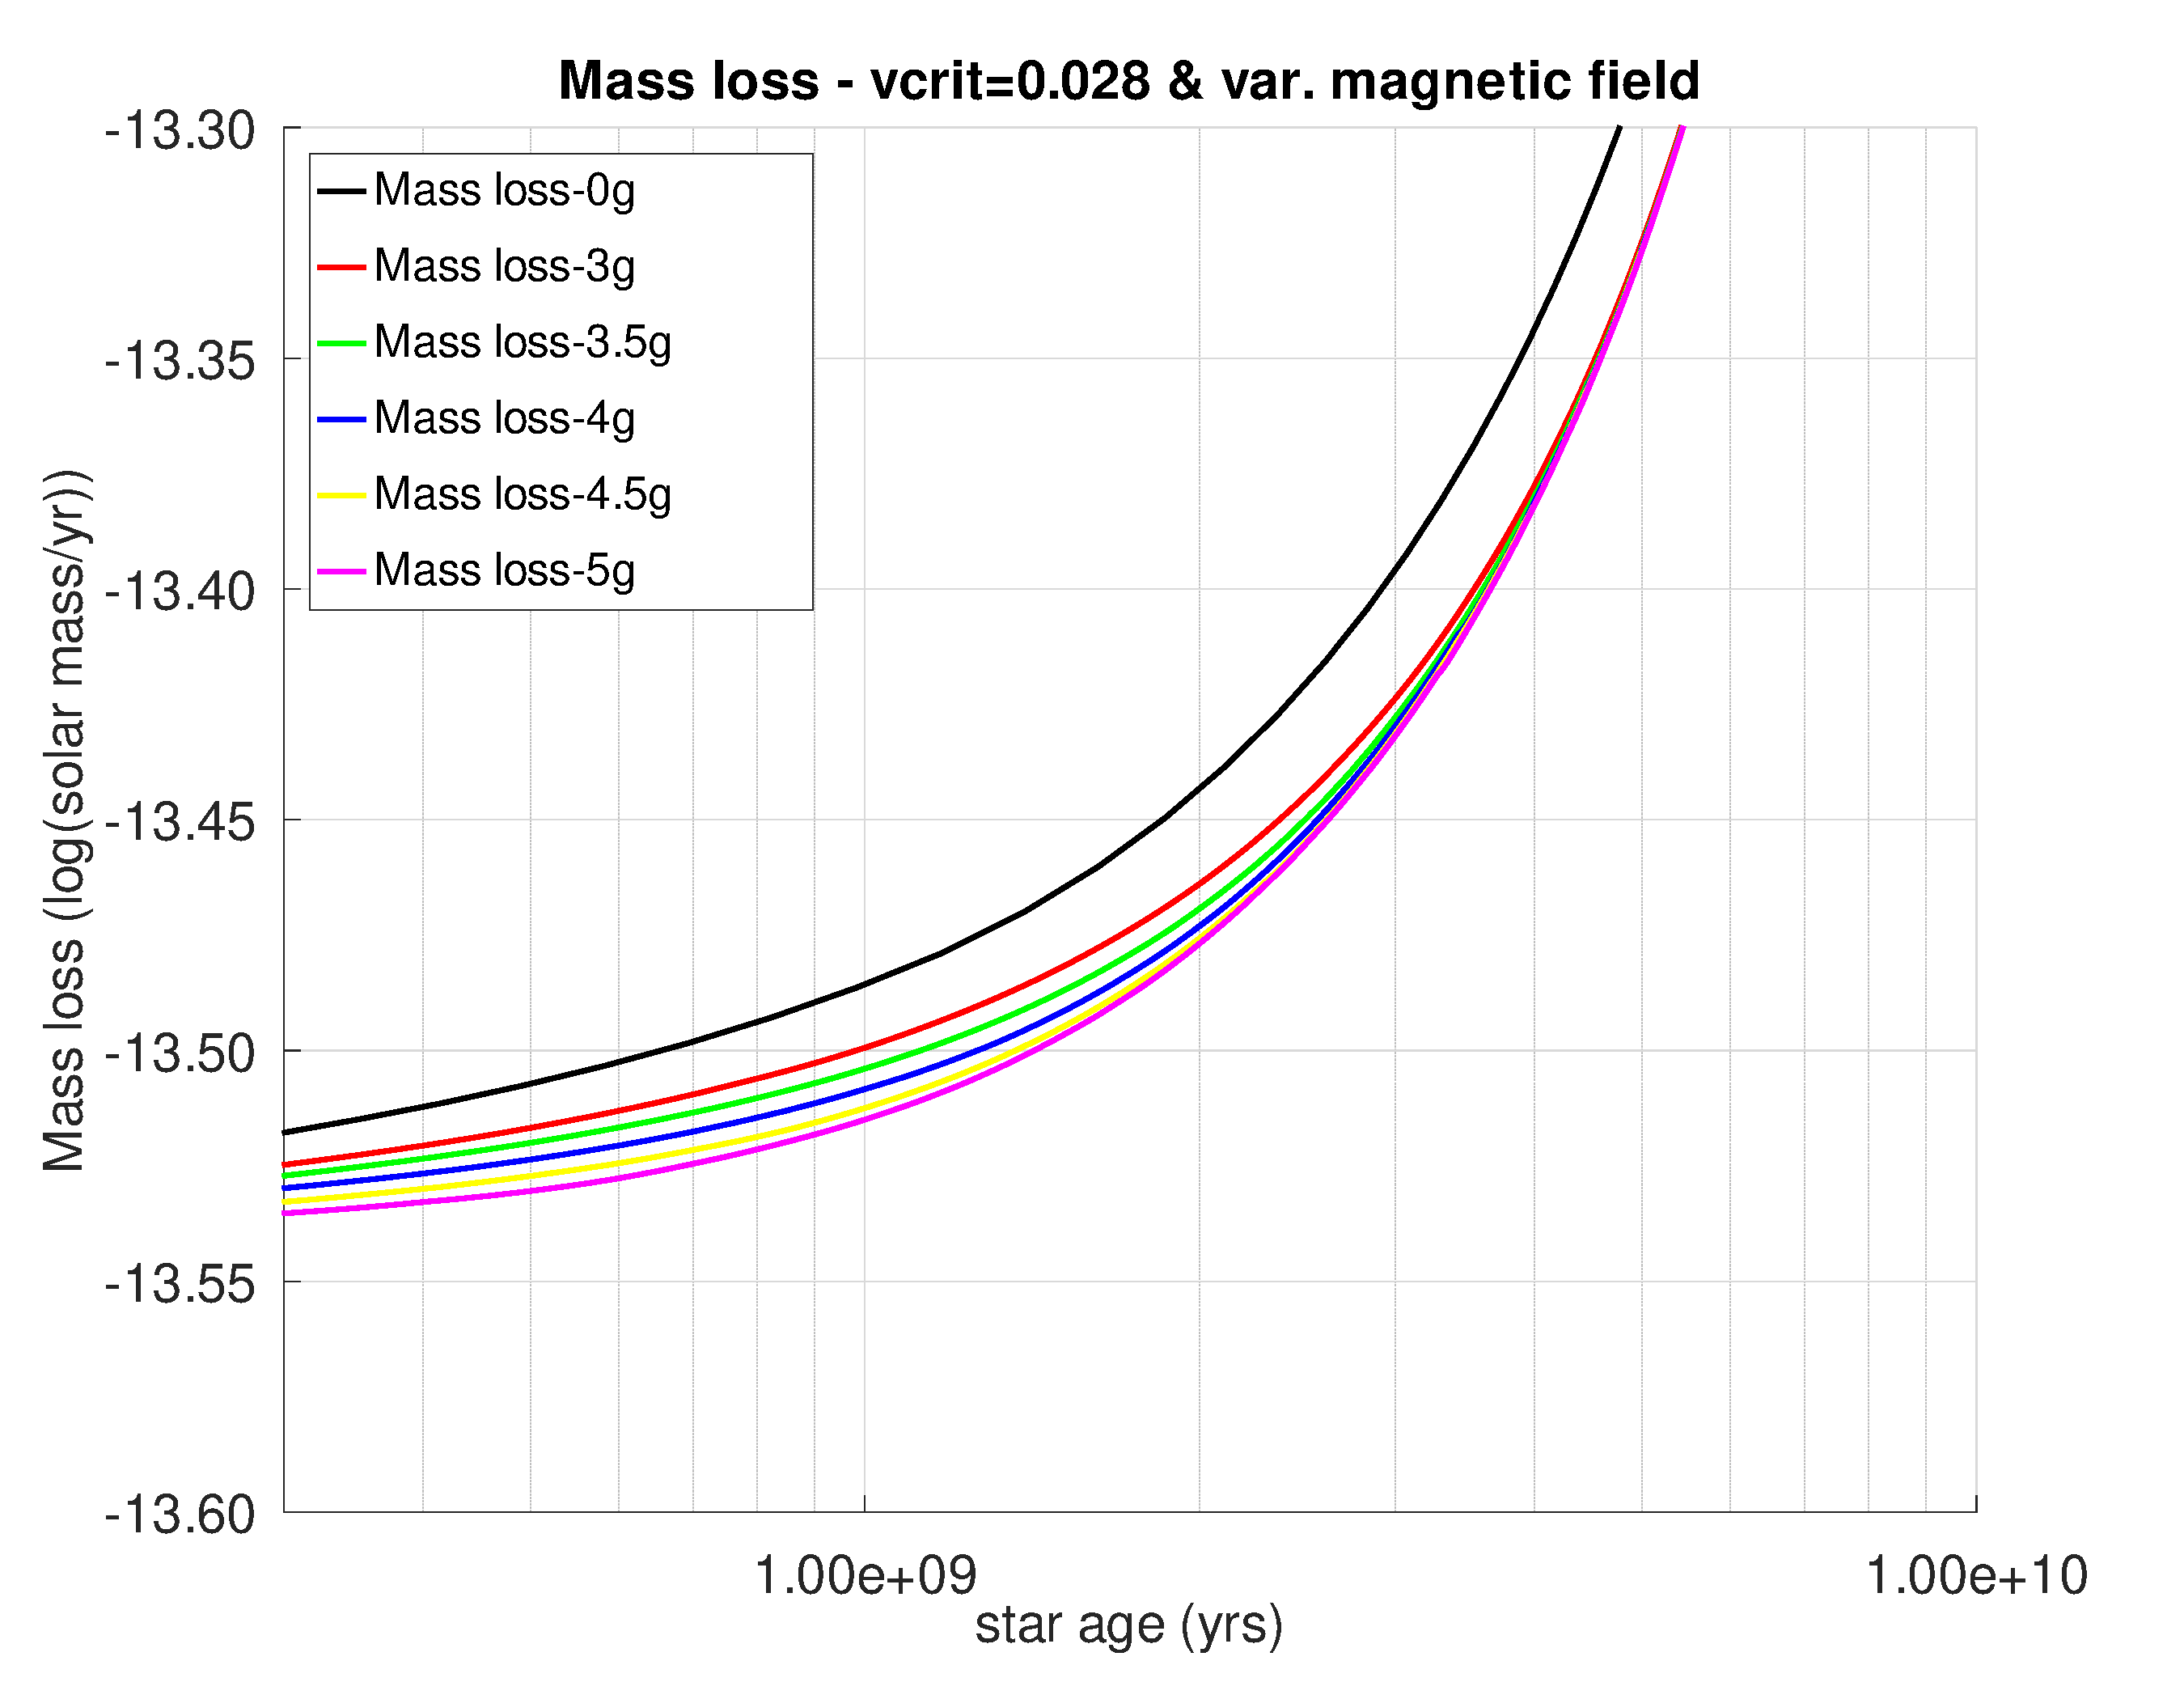
\includegraphics[width=0.7\textwidth]{img/paper1/mdot_vc_028_var_g_z1.pdf}
	\caption{La evolución de la pérdida de masa $\Dot{M}$ a medida que la estrella se acerca a TAMS, en función del tiempo para varios modelos de 1 $\msun$. Los modelos incluyen una intensidad de campo magnético variable entre 0.0G y 5.0G y rotación PMS con $\oomegac=0.028$. Cuanto más intenso sea el campo magnético, menor será $\Dot{M}$.}
	\label{fig:mdot_vc_028_var_b_z1}
\end{figure}

\begin{figure}
    \centering
    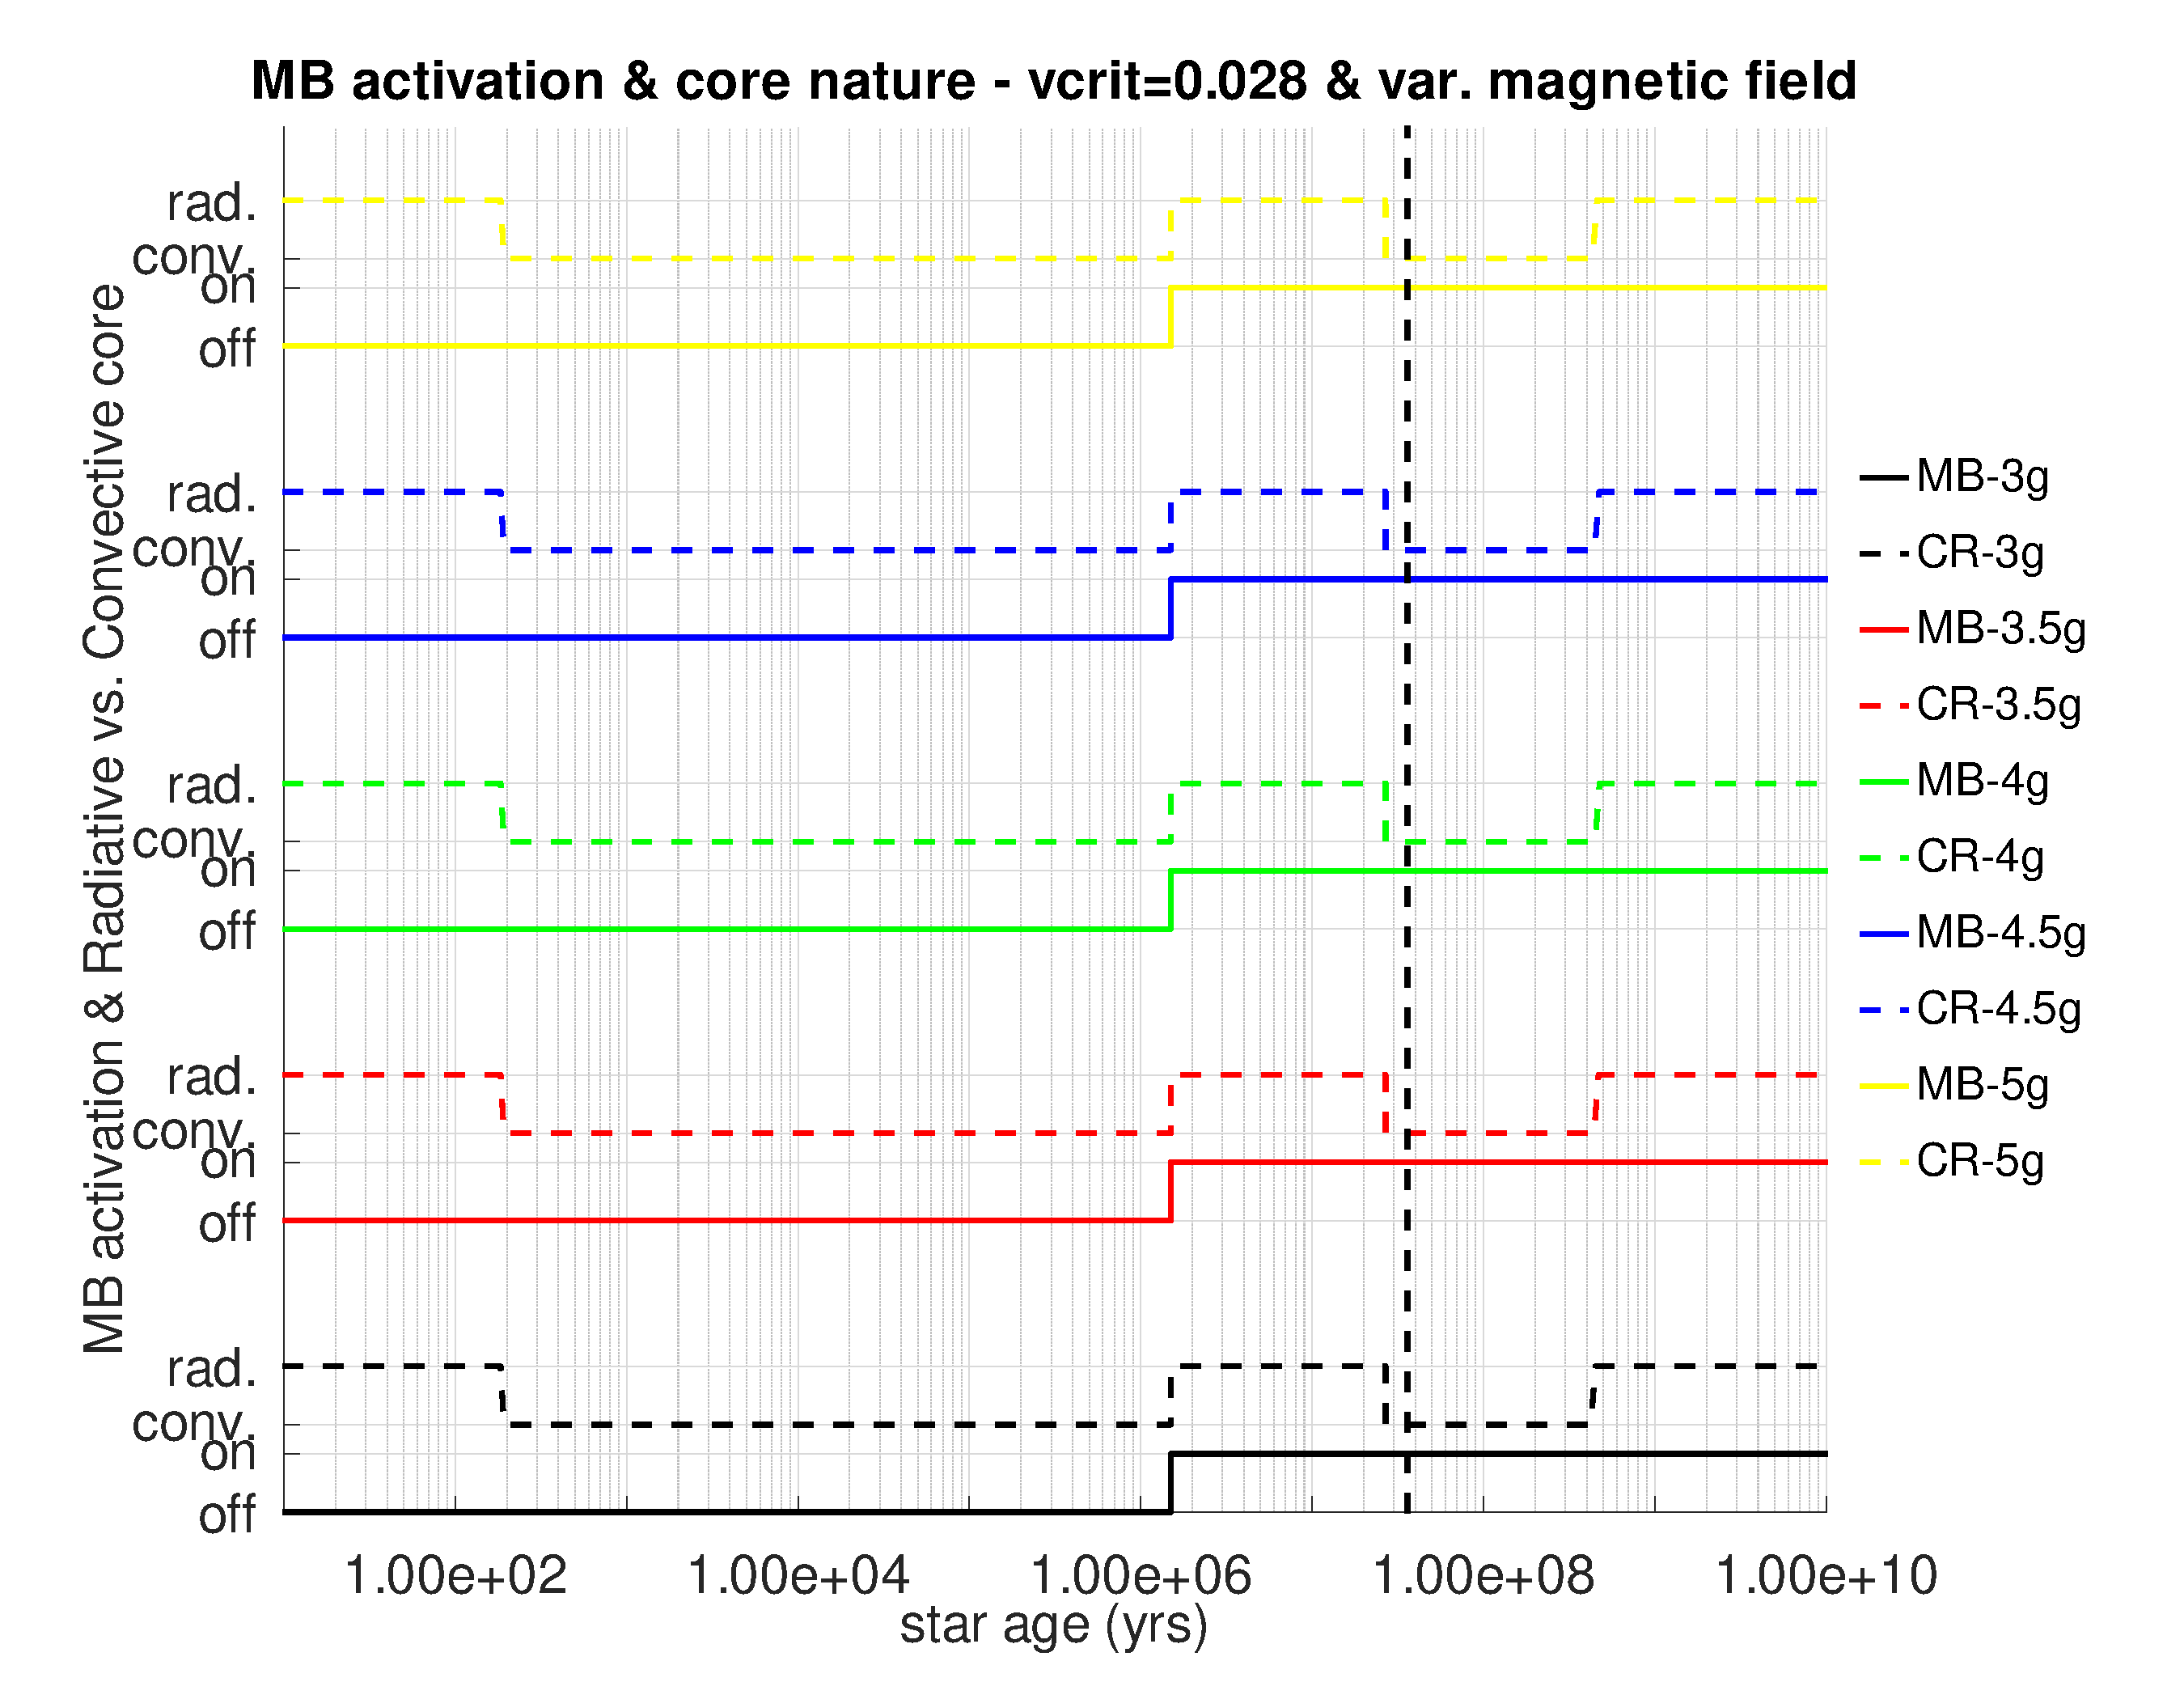
\includegraphics[width=0.7\textwidth]{img/paper1/mb_act_vc_028_var_g.pdf}
	\caption{La activación de la rutina de frenado magnético en función de la presencia de un núcleo radiativo. Los modelos incluyen un campo magnético con una intensidad comprendida entre 0.0G y 5.0G y una rotación PMS con $\oomegac=0.0228$. Las líneas continuas señalan la activación (on) y desactivación (off) de la rutina de frenado magnético. Las líneas horizontales discontinuas informan sobre la naturaleza del núcleo de la estrella: radiativo (rad) o convectivo (conv). Por decisión de implementación, una vez activada la rutina, permanece activada incluso si la naturaleza del núcleo de la estrella cambia a convectiva. La línea vertical discontinua hace referencia a la ZAMS.}
	\label{fig:mb_act_var_vel_vc_028}
\end{figure}

\subsection{Evolución alternativa del Li con MB}
Hasta este punto, las simulaciones de los diferentes modelos se basaron en la parametrización recogida en la Tabla \ref{tab:phy_mesa}, que a su vez fue adoptada de \cite{Choi2016}. Si recordamos la evolución del Li mostrada en las Figuras \ref{fig:li_var_vel_0g} y \ref{fig:li_var_vel_4_0g}, destacamos que en ambos casos se quemaba demasiado Li antes de llegar a la ZAMS y, por tanto, no coincidía con la abundancia media de Li en superficie de las Pléyades. Por otro lado, utilizando una parametrización ligeramente distinta de la empleada hasta ahora en la que los parámetros de convección y \textit{overshooting} se han reajustado según la Tabla \ref{tab:phy_alt_mesa}, las simulaciones pudieron reproducir con mayor fidelidad tanto las abundancias de Li del cúmulo de las Pléyades como las del Sol (véase la Figura \ref{fig:li_3_0g_0314vc}).\par

\begin{table}
	\centering
	\caption{Alternative MTL and overshooting parameters.}
	\label{tab:phy_alt_mesa}
	\begin{tabular}{ll} 
		\hline
		Parameter & Adopted prescriptions and values\\
		\hline
		Convection & MLT + Ledoux, $\alpha_\mathrm{MLT}$ = 1.70\\
		Overshoot & time-dependent, diffusive, $f_\mathrm{ov,core}=0.016$, \\ & $f_\mathrm{ov,sh}=0.002$\\
		\hline
	\end{tabular}
\end{table}

\begin{figure}
    \centering
    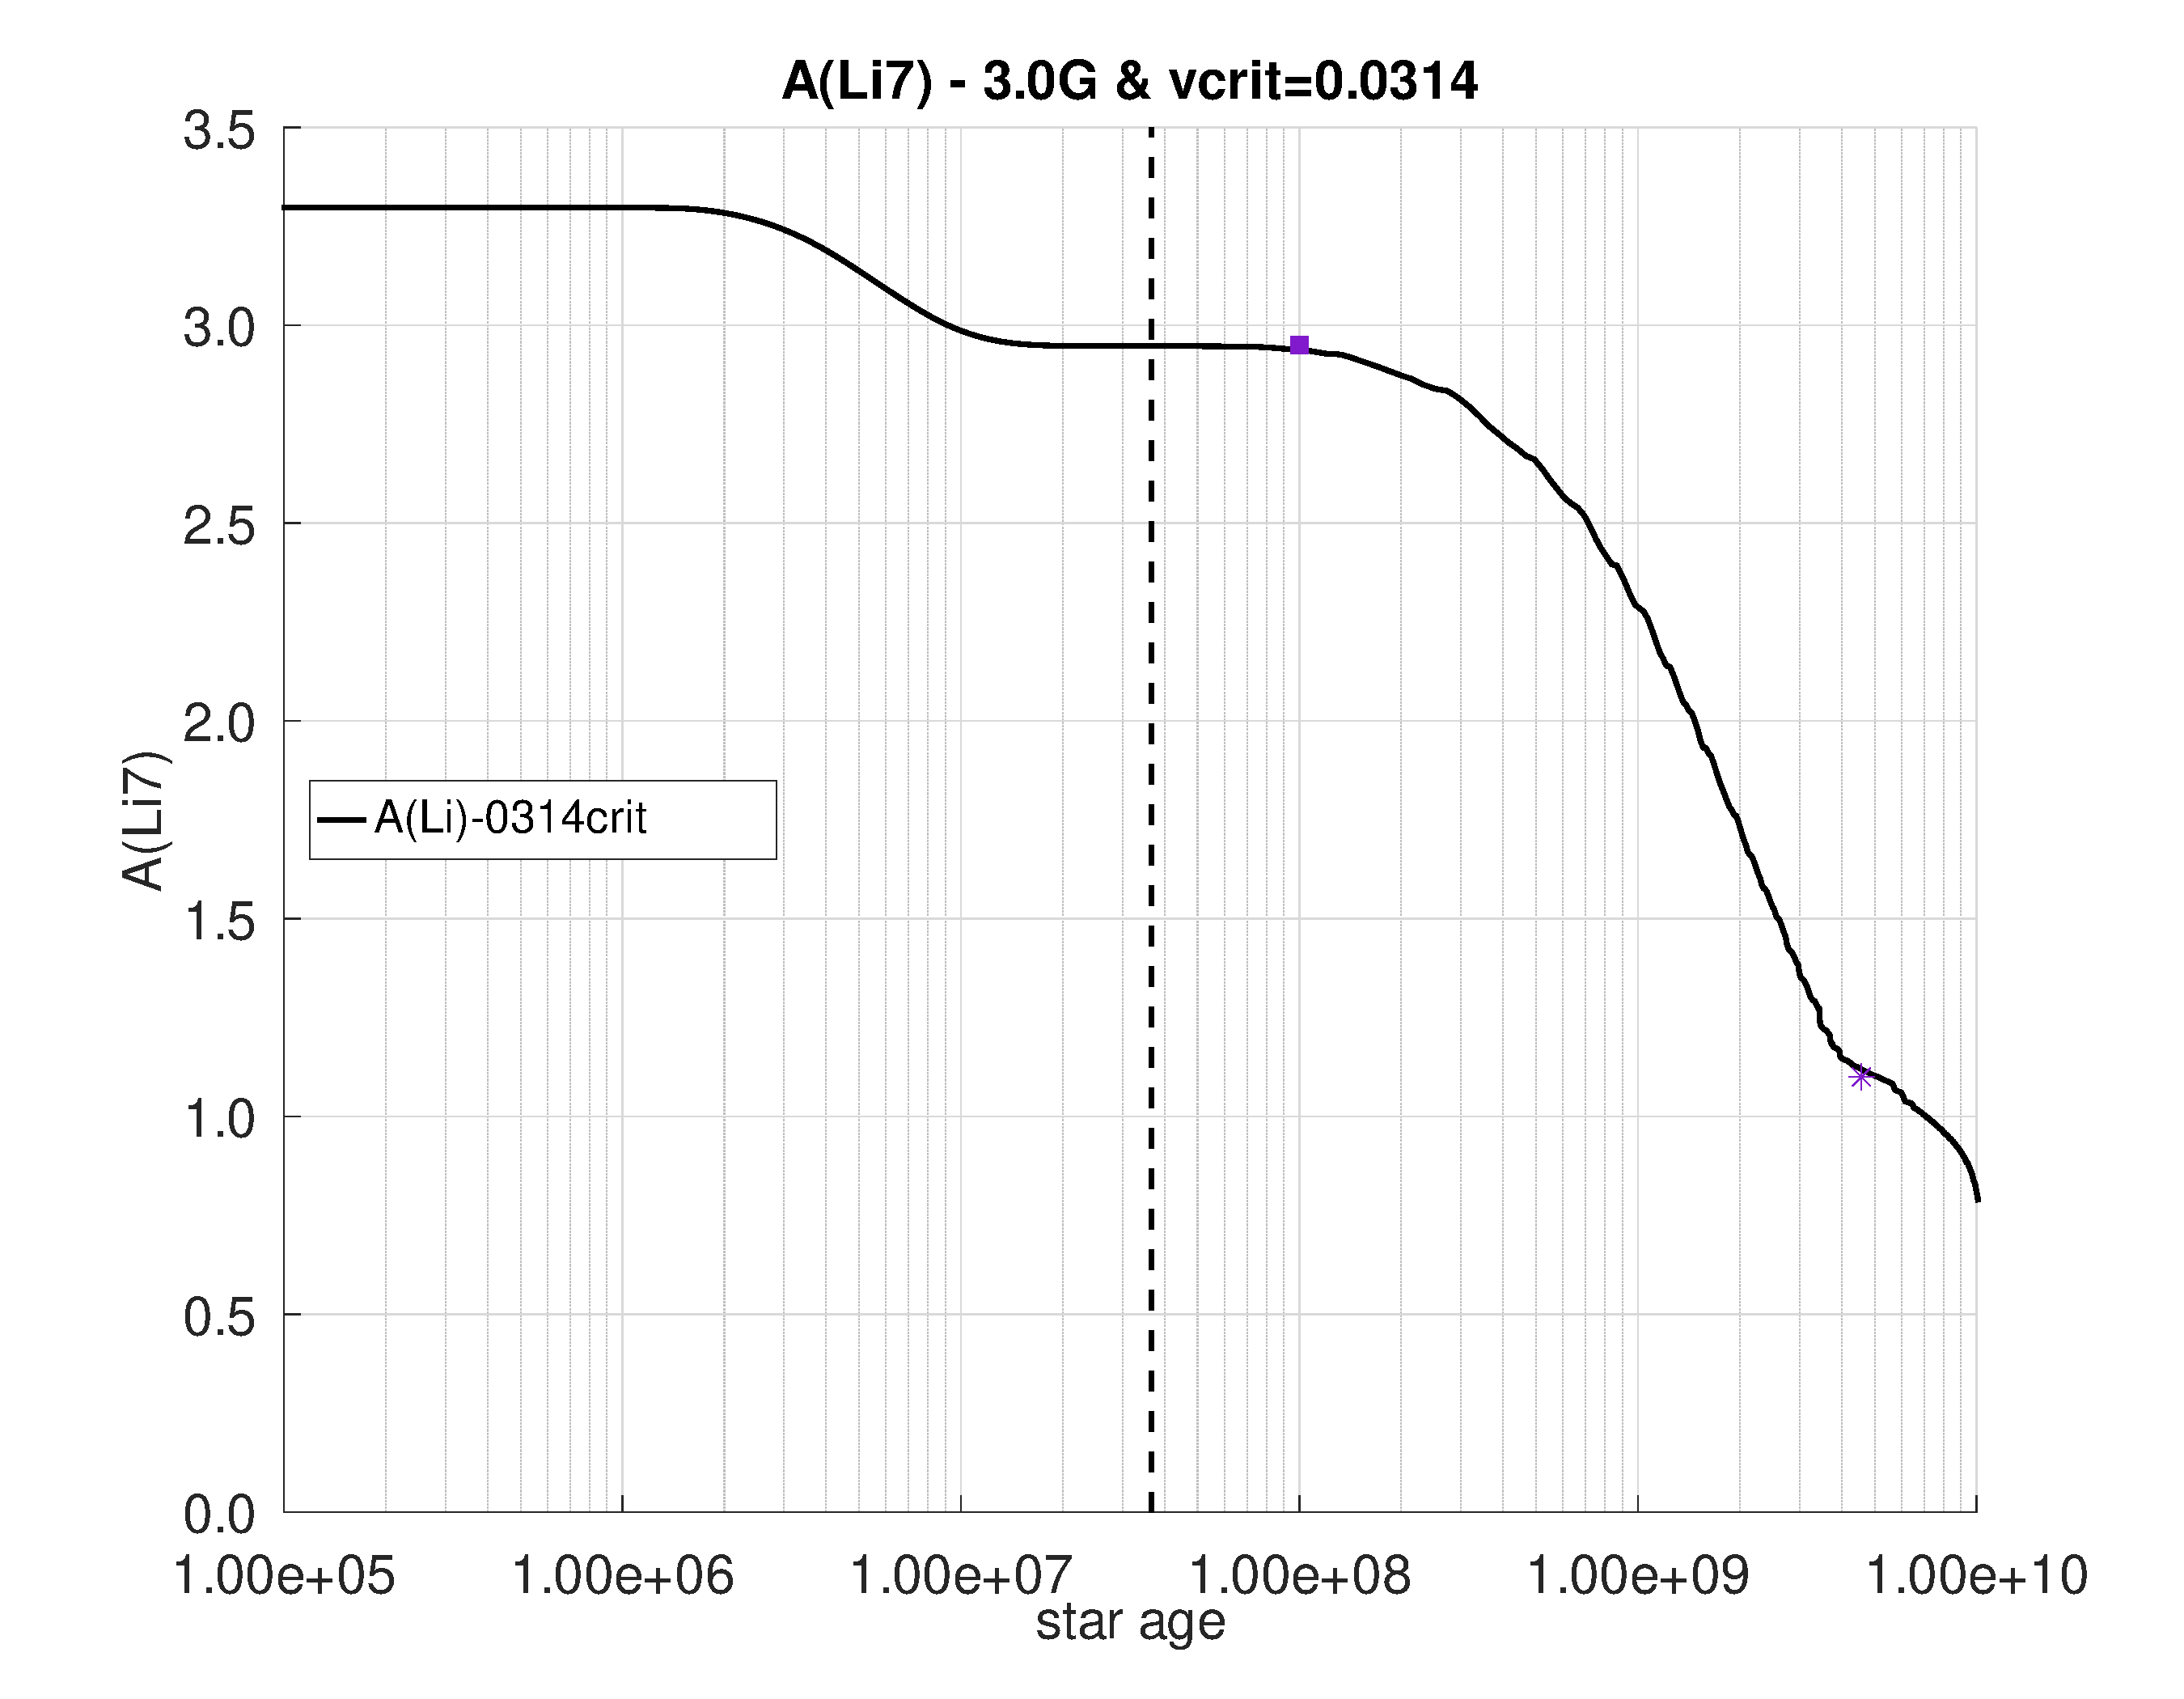
\includegraphics[width=0.7\textwidth]{img/paper1/li_3_0g_0314vc.pdf}
	\caption{La evolución de la abundancia superficial del \isotope[7]{Li} respecto al \isotope[1]{H}, en función del tiempo para un modelo de 1 $\msun$. El modelo incluye un campo magnético con una intensidad de 3G y rotación PMS con $\oomegac= 0.0314$, respectivamente. Los parámetros MLT y overshooting se han fijado en $\alpha_\mathrm{MLT}=1.70$, $f_\mathrm{ov,core}=0.016$, $f_\mathrm{ov,sh}=0.002$. La estrella púrpura y el cuadrado son la abundancia superficial de Li para el Sol actual \cite{Asplund2009} y el cúmulo de las Pléyades \cite{Sestito2005} respectivamente. La línea vertical discontinua hace referencia a la ZAMS.}
	\label{fig:li_3_0g_0314vc}
\end{figure}

Del mismo modo, la evolución de la velocidad angular para esta nueva configuración se muestra en la Figura \ref{fig:rot_vel_var_vel_mlt_3_0g}. Aquí todavía no reproducimos correctamente la velocidad angular del Sol. Se hizo evidente que la influencia de los parámetros libres, relativamente arbitrarios, asociados a MLT condicionaba significativamente la evolución de la abundancia de Li. Sin embargo, sin la inclusión de MB no fue posible ajustarlo para las Pléyades y el Sol con la misma trayectoria evolutiva. Este hecho abre la puerta a otras parametrizaciones compatibles con el Sol para reproducir las observaciones en cúmulos estelares jóvenes y para el Sol.\par

\begin{figure}
    \centering
    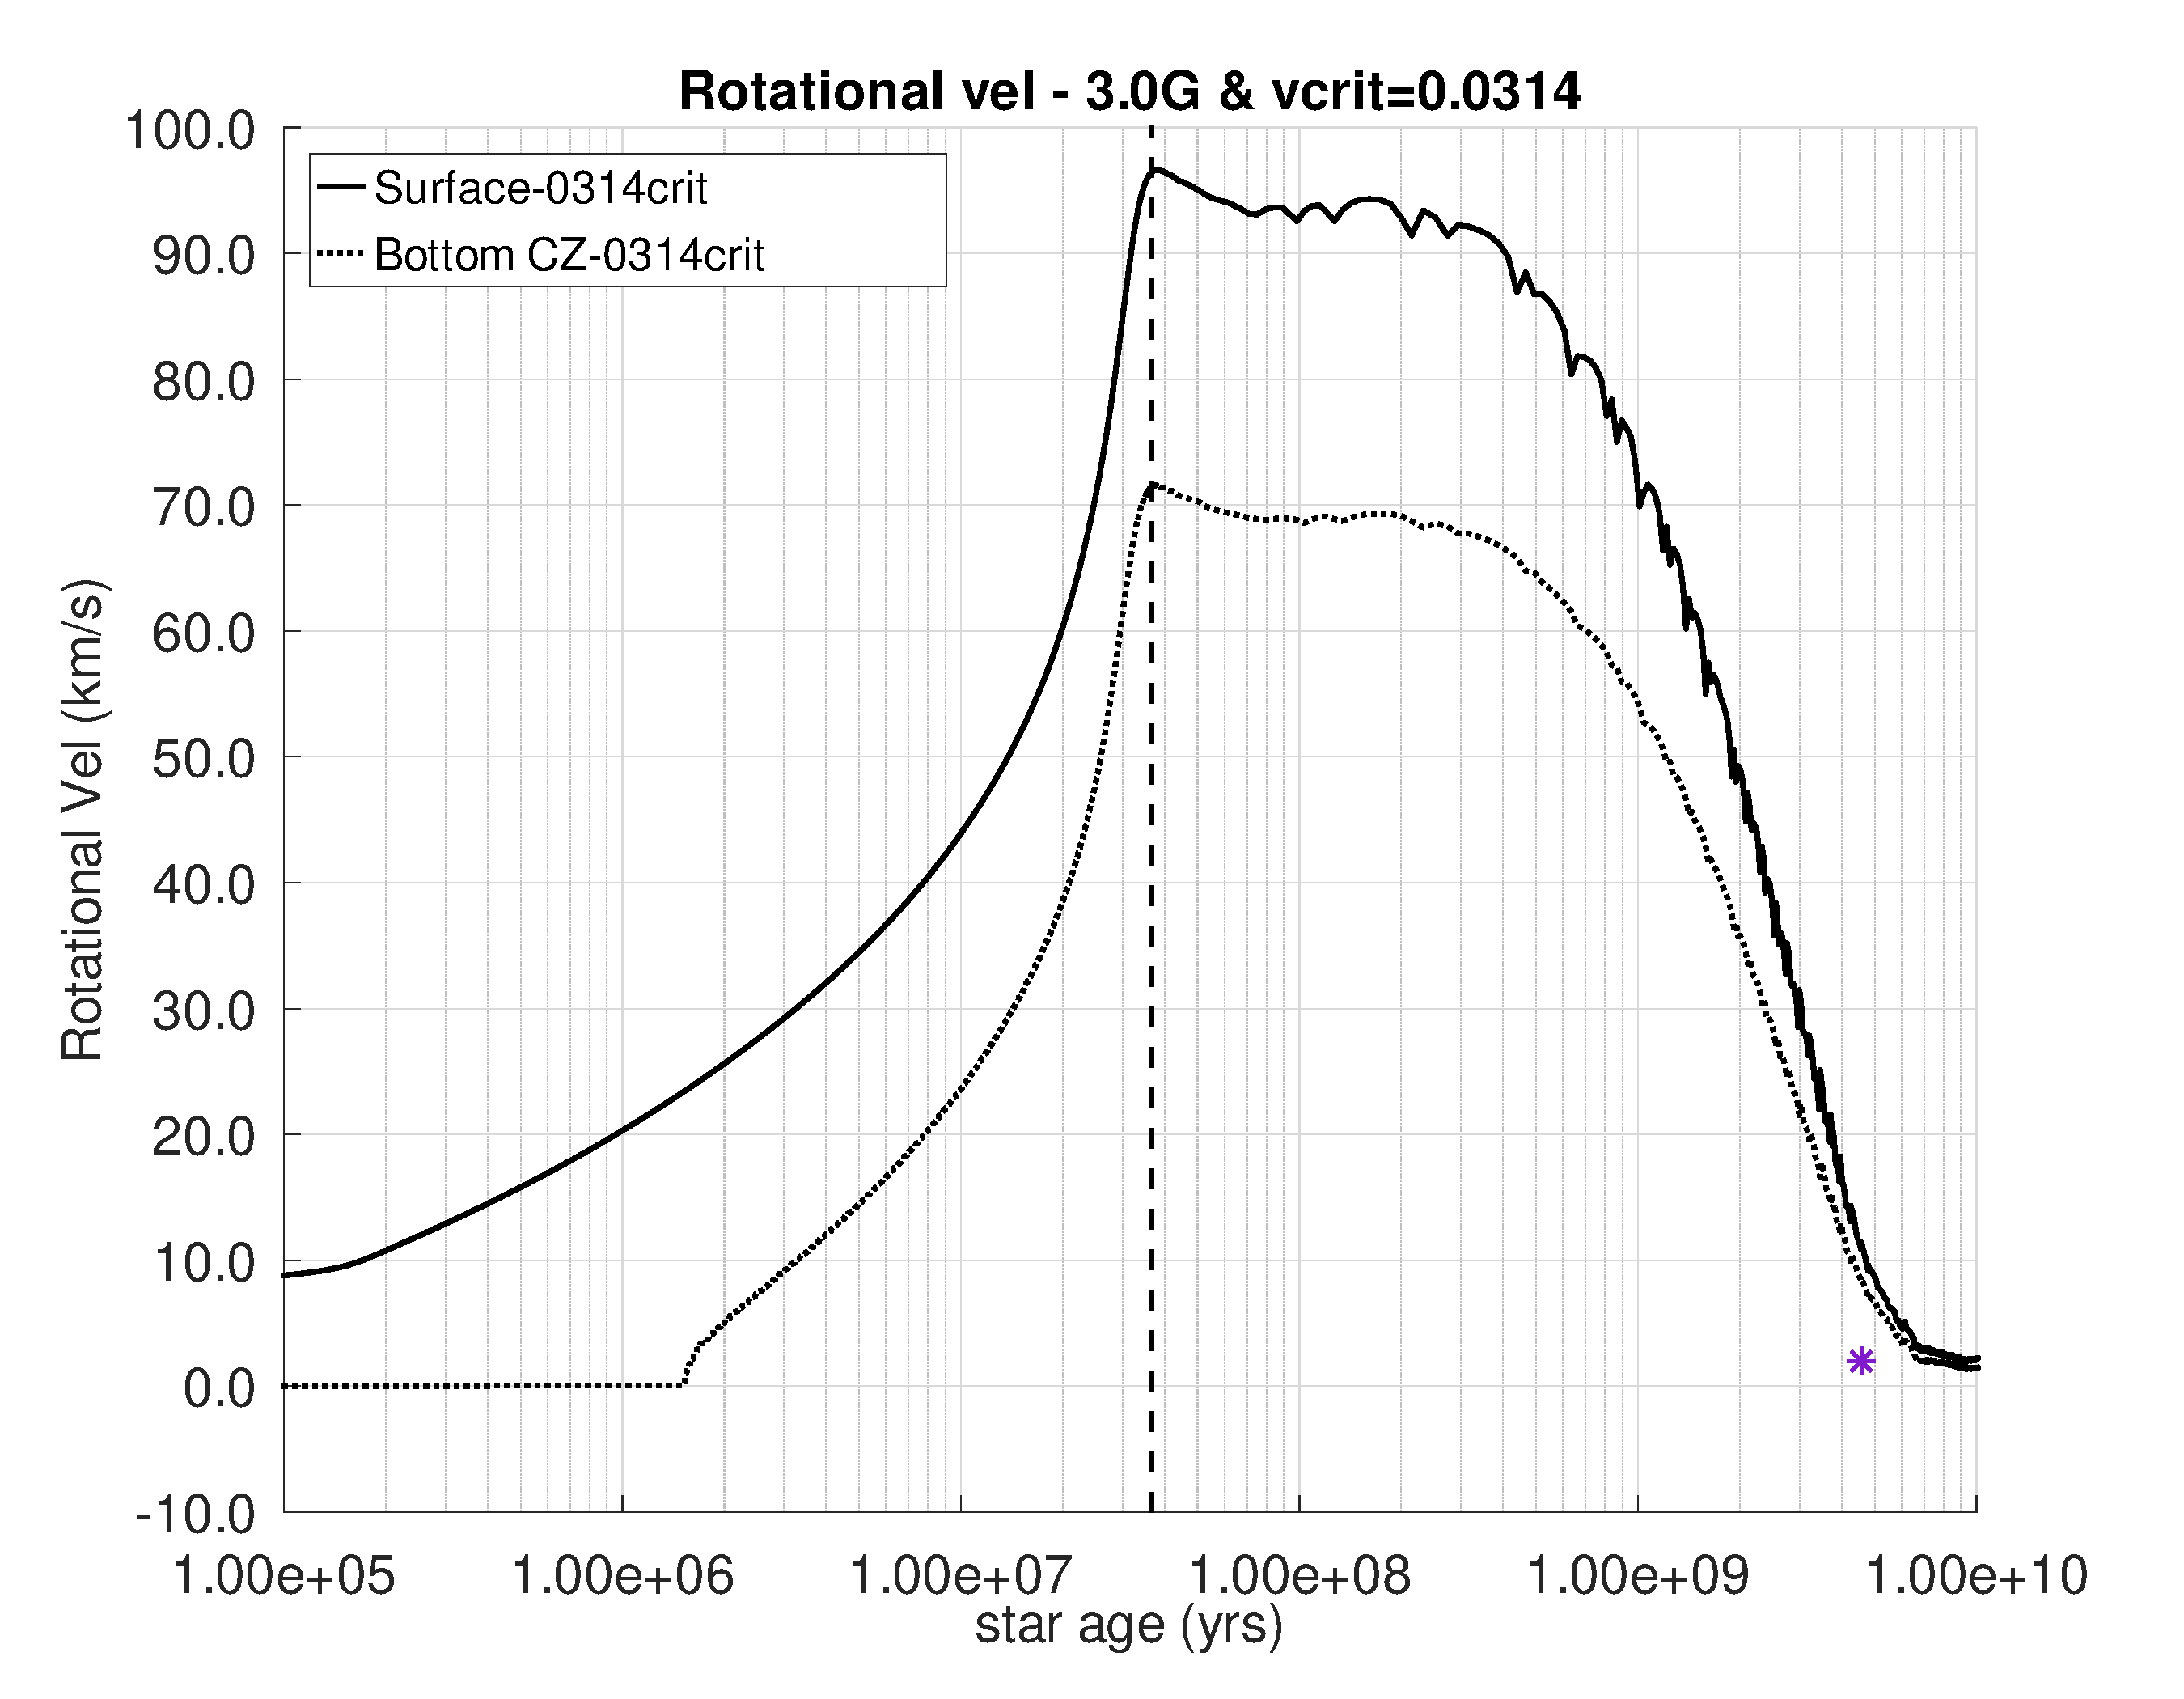
\includegraphics[width=0.7\textwidth]{img/paper1/rot_vel_3_0g_0314vc.pdf}
	\caption{La evolución de la velocidad de rotación de la superficie, en función del tiempo para un modelo de 1 $\msun$. El modelo incluye un campo magnético con una intensidad de 3G, rotación PMS con $\oomegac=0.0314$, parámetros en la Tabla \ref{tab:phy_alt_mesa} y MB. La estrella púrpura es la velocidad angular superficial para el Sol actual \cite{Gill2012}. La línea vertical discontinua hace referencia a la ZAMS.}
	\label{fig:rot_vel_var_vel_mlt_3_0g}
\end{figure}

\section{Conclusiones} \label{sec_conclusions}
Hemos demostrado, a través de los diferentes modelos estelares simulados, que los efectos inducidos por la combinación de ambos mecanismos de rotación y frenado magnético ofrecen una forma plausible de reconciliar los datos observacionales con los modelos teóricos. Esto último es de gran importancia tanto para el transporte de AM como para el transporte de elementos químicos. También somos muy conscientes de que aún estamos lejos de comprender los mecanismos físicos exactos que gobiernan estos procesos, por lo que es necesario seguir profundizando en estas áreas de estudio. En particular, el estudio de la evolución de los campos magnéticos durante la PMS y la MS, y su impacto en la AML. \par

Se realizarán futuras y mejoradas implementaciones de nuestra rutina para estudiar los resultados sobre las huellas, la composición superficial del Li, la rotación, etc. Es probable que en un modelo estelar en rotación simulado con MB desde el principio, la rotación diferencial sea muy reducida y, por tanto, las abundancias de Li observadas en estrellas jóvenes podrían explicarse adecuadamente. Proponemos que este resultado podría alcanzarse mediante una ley de interdependencia entre $\Omega$ y $B$. Así, durante el PMS, cuando la estrella rota más rápido, el efecto MB es más eficiente. En cambio, durante el MS, cuando el arranque se ralentiza, el MB será menos intenso. Este enfoque establecería un mecanismo de autorregulación sobre la velocidad angular de la estrella que acabaría influyendo directamente en la evolución del Li. Es igualmente importante comprender mejor el papel general de la pérdida de masa en AML y sobre todo en estrellas más frías y de baja masa. Hoy en día es un reto determinar la velocidad terminal del viento estelar para este tipo de estrellas que juega un papel clave en la AML.\par

Subrayamos también que nuestros modelos no coincidieron al mismo tiempo con la abundancia de Li solar observada y $\Omega$. Por lo tanto, no podemos asegurar que hayamos modelado correctamente la historia rotacional del Sol. En vista de estas deficiencias de nuestros modelos, debemos analizar los resultados obtenidos con cautela y no sacar conclusiones prematuras. También hemos mostrado cómo una parametrización MLT alternativa podría producir resultados acordes con las observaciones. En el transcurso de este trabajo se han apoyado las siguientes conclusiones:
\begin{enumerate}
	\item La inclusión del campo magnético conduce a modelos más fríos y a un menor agotamiento de Li en la EM.
	\item Una combinación de rotación durante la PMS y efecto MB durante la MS produce un comportamiento diferente y potencialmente más prometedor que los producidos por los modelos estándar. Así, nuestro enfoque apunta a reproducir el A(Li) observado y la velocidad de rotación solar al mismo tiempo.
	\item $\teff$ de las trayectorias evolutivas estándar representan límites superiores, ya que estos modelos no tienen en cuenta el efecto de frenado magnético ni la rotación.
	\item La extensión de la zona convectiva disminuye cuando aumenta la intensidad del campo magnético.
	\item El MB durante la PMS y/o el ajuste de los parámetros libres de exceso de MLT y $\amlt$ parece ser también necesario para explicar las abundancias de Li en cúmulos jóvenes.
\end{enumerate}

\endinput
%--------------------------------------------------------------------
% FIN DEL CAPÍTULO. 
%--------------------------------------------------------------------
